\documentclass[12pt,a4paper,oneside]{report}

% ---------- Encoding & Language ----------
\usepackage[utf8]{inputenc}
\usepackage[T1]{fontenc}
\usepackage[french,english]{babel}
\usepackage{csquotes}
\usepackage{microtype}

% ---------- Page & Typography ----------
\usepackage{geometry}
\geometry{margin=2.5cm}
\usepackage{setspace}
\onehalfspacing

% ---------- Maths, Tables, Figures ----------
\usepackage{amsmath,amssymb}
\usepackage{siunitx}
\sisetup{detect-all,round-mode=places}
\usepackage{graphicx}
\usepackage{subcaption}
\usepackage{booktabs}
\usepackage{caption}
\usepackage{longtable}
\captionsetup{labelfont=bf}
\usepackage{multirow}



% ---------- Links & Clever refs ----------
\usepackage{hyperref}
\hypersetup{
  colorlinks=true,
  linkcolor=blue,
  citecolor=blue,
  urlcolor=blue,
  pdftitle={Mémoire de stage},
  pdfauthor={Magaye Ndiaye}
}
\usepackage[nameinlink,noabbrev]{cleveref}

% ---------- TikZ for pipeline diagram ----------
\usepackage{tikz}
\usetikzlibrary{arrows.meta,positioning,fit,shapes.geometric,calc}

% ---------- Acronyms (optional) ----------
\usepackage[acronym]{glossaries}
\makeglossaries

% ---------- Bibliography ----------
% \usepackage[
%   backend=biber,
%   style=authoryear,
%   maxbibnames=8,
%   maxcitenames=2,
%   giveninits=true,
%   uniquename=false
% ]{biblatex}
% \addbibresource{references.bib}
\usepackage[
  backend=biber,
  style=numeric,        % style de biblio : [1], [2], ...
  citestyle=numeric-comp, % compresse les séries : [1–3,5]
  sorting=none,         % ordre d’apparition dans le texte
  giveninits=true,      % initiales pour les prénoms
  maxbibnames=8,        % nb. max d'auteurs listés
  doi=true,
  url=true
]{biblatex}
\addbibresource{references_tools_institutions.bib}

% ---------- Custom commands ----------
\newcommand{\Rtwo}{\ensuremath{R^2}}
\newcommand{\RMSE}{\ensuremath{\mathrm{RMSE}}}

% ---------- Acronyms list (edit as needed) ----------
\newacronym{soc}{SOC}{Soil Organic Carbon}
\newacronym{gee}{GEE}{Google Earth Engine}
\newacronym{dem}{DEM}{Digital Elevation Model}
\newacronym{ml}{ML}{Machine Learning}
\newacronym{rf}{RF}{Random Forest}
\newacronym{gbm}{GBM}{Gradient Boosting Machine}
\newacronym{mlp}{MLP}{Multi-Layer Perceptron}
\newacronym{api}{API}{Application Programming Interface}

% ---------- Title page ----------
\title{\textbf{Prédiction du stock de carbone organique du sol}\\
\large Application aux villages de Bary, Diohine/Sassem et Sop}
\author{Magaye Ndiaye}
\date{Avril -- Septembre 2025}

\begin{document}
\selectlanguage{french}
\pagenumbering{roman}
% ---------- Page de garde ----------
\begin{titlepage}
\begin{center}

% Logos en haut
\begin{minipage}{0.3\textwidth}
  
\includegraphics[width=\linewidth]{images/university-of-bordeaux_logo.png}
\end{minipage}
\hfill
\begin{minipage}{0.3\textwidth}
  \centering
  
\includegraphics[width=0.8\linewidth]{images/logo_ird.png}
\end{minipage}
\hfill
\begin{minipage}{0.3\textwidth}
  \raggedleft
  \includegraphics[width=\linewidth]{images/logo_ummisco.png}
\end{minipage}

\vspace{2cm}

% Titre
{\Large \textbf{Mémoire de Master}} \\[0.5cm]
{\large Master Informatique – Parcours Intelligence artificielle}\\[1.2cm]

{\Huge \textbf{Prédiction du stock de carbone organique du sol}}\\[0.3cm]
{\Large Application aux villages de Bary, Diohine/Sassem et Sop}\\[2cm]

% Auteur
\textbf{Présenté par :} \\
{\large Magaye Ndiaye}\\[1cm]

% Encadrants
\textbf{Encadrants :} \\
Dr. Mandicou Ba (UMMISCO, IRD) \\
Pr. Marie Beurton-Aimar (Université de Bordeaux) \\[2cm]

% Dates
{\large Avril – Septembre 2025}\\[3cm]

% Pied de page
\textit{Université de Bordeaux – Institut de Recherche pour le Développement (IRD) – UMMISCO Sénégal}

\end{center}
\end{titlepage}


\chapter*{Remerciements}
\begin{flushleft}
Je tiens tout d’abord à exprimer ma profonde gratitude à Dieu Tout-Puissant pour m’avoir donné la force, la santé et la persévérance nécessaires à la réalisation de ce mémoire.

Je remercie sincèrement mon encadrant Dr. Mandicou Ba pour son accompagnement bienveillant, ses conseils éclairés et son exigence scientifique, qui ont été essentiels à la bonne conduite de ce travail. J’adresse également mes remerciements à Professeure Marie Beurton-Aimar et à M. Zemmari pour leur disponibilité, leurs encouragements et leurs orientations précieuses.

Mes remerciements vont également à l’ensemble de l’équipe de l’UMMISCO Sénégal et du projet SLAM-B, pour l’accueil chaleureux et l’environnement scientifique stimulant qu’ils m’ont offert durant ce stage.

Je souhaite aussi exprimer ma reconnaissance au programme Numerics de l’Université de Bordeaux, qui m’a permis de bénéficier d’un cadre de formation académique de haut niveau et de ressources précieuses pour la réalisation de ce travail.

Je n’oublie pas mes camarades et collègues de recherche, dont les échanges m’ont permis d’enrichir mes réflexions et d’élargir mes horizons.

Enfin, j’adresse une pensée particulière à ma famille et à mes proches, pour leur soutien moral et affectif constant. Leur confiance et leurs encouragements m’ont donné la motivation de toujours aller de l’avant.
\end{flushleft}
\vspace{2cm}

\begin{abstract}
\textbf{Résumé ---}\noindent Le carbone organique du sol (SOC) est un levier central pour la fertilité, la rétention en eau et l’atténuation du changement climatique. Dans le contexte sahélien, la variabilité pluviométrique, l’érosion et la pression anthropique exigent des outils de cartographie fiables et reproductibles. Ce travail propose un pipeline de prédiction du SOC dans trois villages du centre du Sénégal (Bary, Diohine/Sassem, Sop) combinant données pédologiques (AfSP et IRD), télédétection optique (Sentinel-2, Landsat-8) et apprentissage automatique. Les images ont été filtrées et agrégées en composites trimestriels (2013–2025 pour Landsat-8 ; 2015–2025 pour Sentinel-2), puis enrichies en indices spectraux (NDVI, NDWI, BSI, CI-Green) et en covariables topographiques et pédologiques globales. Plusieurs modèles ont été entraînés (RF, Gradient Boosting, XGBoost, HistGradientBoosting, MLP PyTorch) sous validation stricte par groupes (GroupKFold) afin de limiter les fuites spatiales. Les meilleurs résultats sont obtenus avec un MLP (stacking en appui), avec des performances atteignant \textit{R\textsuperscript{2} = 0.80} et \textit{RMSE = 0.52 g/kg} pour 0–10 cm, et \textit{R\textsuperscript{2} = 0.65} et \textit{RMSE = 0.66 g/kg} pour 10–30 cm. Des cartes d’incertitude (écart-type et intervalles à 90\,\%) accompagnent les cartes prédictives pour appuyer la décision et orienter de futures campagnes terrain. Enfin, nous discutons les limites (synchronisation temporelle données sol / satellites, hétérogénéités locales) et proposons des pistes d’amélioration (hybrides géostatistiques, capteurs complémentaires, enrichissement des données locales).
\par\smallskip
\textbf{Mots-clés :} carbone organique du sol ; télédétection ; Sentinel-2 ; Landsat-8 ; apprentissage automatique.
\end{abstract}

\selectlanguage{english}
\begin{abstract}

\textbf{Abstract ---} \noindent
Soil Organic Carbon (SOC) underpins soil fertility, water retention and climate mitigation. In the Sahel, strong rainfall variability, erosion and human pressure call for reliable and reproducible SOC mapping tools. We design a prediction pipeline for three villages in central Senegal (Bary, Diohine/Sassem, Sop) that blends soil observations (IRD), optical remote sensing (Sentinel-2, Landsat-8) and machine learning. Satellite archives are quality-filtered and aggregated into quarterly composites (2013–2025 for Landsat-8; 2015–2025 for Sentinel-2) and complemented with spectral indices (NDVI, NDWI, BSI, CI-Green) plus topographic and global soil covariates. We train multiple models (RF, Gradient Boosting, XGBoost, HistGradientBoosting, PyTorch MLP) under strict group-based validation (GroupKFold) to avoid spatial leakage. The best performance is achieved by an MLP (with stacking support), reaching \textit{R\textsuperscript{2} = 0.80} and \textit{RMSE = 0.52 g/kg} at 0–10 cm, and \textit{R\textsuperscript{2} = 0.65} and \textit{RMSE = 0.66 g/kg} at 10–30 cm. Predictive maps are paired with uncertainty layers (standard deviation and 90\% confidence intervals) to guide decisions and plan additional field sampling. We discuss limitations (temporal alignment between soil and satellite data, local heterogeneity) and outline improvements (hybrid geostatistical methods, complementary sensors, and richer local datasets).
\par\smallskip
\textbf{Keywords:} soil organic carbon; remote sensing; Sentinel-2; Landsat-8; machine learning.
\end{abstract}
\selectlanguage{french}

\tableofcontents
\listoffigures
\listoftables

\printglossary[type=\acronymtype,title=Liste des acronymes]

\cleardoublepage
\pagenumbering{arabic}

% =================== Chapitre 1 ====================
\chapter{Introduction}

\section{problématique et contexte}
Le carbone organique du sol (SOC) joue un rôle fondamental dans la fertilité\cite{minasny_soil_2017}, la régulation hydrique et l’atténuation du changement climatique. Dans les zones sahéliennes, et en particulier au Sénégal, la pression agricole sur les terres du bassin arachidier, combinée à une forte variabilité pluviométrique et à l’érosion, menace la durabilité des systèmes de production. Or, le suivi du SOC constitue un levier majeur pour améliorer la productivité agricole, préserver les ressources en eau et contribuer aux engagements climatiques internationaux.
Malgré son importance, la cartographie du SOC reste complexe. Les mesures directes par prélèvements et analyses en laboratoire sont précises, mais elles demeurent coûteuses, chronophages et spatialement limitées. En parallèle, la télédétection et l’apprentissage automatique offrent aujourd’hui des alternatives puissantes pour estimer et cartographier le SOC à grande échelle, mais leur mise en œuvre en contexte sahélien reste encore peu explorée.
\\
\newline
Dans ce cadre, il est crucial de concevoir des outils de prédiction fiables, reproductibles et adaptés aux réalités locales, afin de fournir des cartes utiles aux chercheurs, décideurs et agriculteurs.

\section{Carbone organique du sol}

\subsection{Cycle du carbone et puits de carbone}
Le SOC représente un compartiment essentiel du cycle global du carbone\cite{minasny_soil_2017}. Il agit comme un puits de carbone, en stockant une partie du CO$_2$ atmosphérique sous forme de matière organique. La dynamique de ce stockage dépend des pratiques agricoles, des conditions climatiques et des propriétés physico-chimiques des sols.

\subsection{Rôle du SOC dans les écosystèmes}
Au-delà de son rôle climatique, le SOC conditionne la structure du sol, sa porosité et sa capacité de rétention en eau. Il favorise la productivité agricole en soutenant la fertilité et en renforçant la résilience des sols face aux stress climatiques (sécheresse, érosion). La dégradation du SOC entraîne au contraire un appauvrissement des sols et une vulnérabilité accrue des systèmes agricoles.

\subsection{Séquestration du carbone}
La séquestration \cite{lal_soil_2004} du carbone organique dans les sols est un levier d’atténuation du changement climatique. Des pratiques telles que les rotations culturales, l’agroforesterie, l’apport de résidus organiques ou le maintien de couvertures végétales permettent d’accroître les stocks de SOC. Toutefois, ces gains restent hétérogènes dans l’espace et se matérialisent lentement, ce qui rend nécessaire le suivi spatial et temporel du SOC à haute résolution.
Les pratiques de gestion durable des terres, telles que l'agroforesterie, la couverture végétale et l'application de matières organiques, peuvent favoriser la séquestration du carbone dans le sol. Cependant, les gains en matière de SOC sont souvent lents à se matérialiser et varient considérablement en fonction des contextes locaux.


\section{Objectifs scientifiques et originalité du travail}

L’objectif général de ce stage est de concevoir un pipeline opérationnel et reproductible pour estimer et cartographier le SOC (0–10 cm et 10–30 cm) dans trois villages pilotes du centre du Sénégal (Bary, Diohine/Sassem et Sop).

Plus spécifiquement, ce travail vise à :
\begin{itemize}


\item Intégrer des données multi-sources : profils pédologiques (AfSP, IRD, WoSIS), imagerie satellitaire optique (Sentinel-2, Landsat-8), indices spectraux et covariables environnementales (topographie, sols globaux).

\item Évaluer plusieurs approches de modélisation : géostatistique, méthodes d’apprentissage automatique (forêts aléatoires, boosting) et réseaux de neurones (MLP PyTorch), avec une validation rigoureuse par groupes pour limiter les fuites spatiales.

\item Cartographier l’incertitude associée aux prédictions, afin de fournir aux utilisateurs non seulement une estimation du SOC mais aussi un indicateur de fiabilité.

\item Déployer une application web interactive (Django/PostGIS) intégrant une API de prédiction et une interface cartographique pour rendre les résultats accessibles aux chercheurs et décideurs.
\end{itemize}

\section{Conclusion}
Cette introduction met en évidence l’importance du SOC dans la fertilité des sols et la lutte contre le changement climatique, tout en soulignant les limites des approches classiques de mesure. Elle justifie le recours à la télédétection et à l’apprentissage automatique pour développer des outils adaptés au contexte sahélien.\\
\newline
Le chapitre suivant présentera un état de l’art sur les approches existantes de cartographie du SOC, les données mobilisées (profils pédologiques, télédétection), ainsi que les principaux projets et travaux antérieurs qui ont inspiré et guidé ce mémoire.


% ===================== Chapitre 1,2 =====================

\chapter{État de l’art}

\section{Concepts et enjeux}
La mesure directe du SOC repose sur des prélèvements de sol suivis d’analyses en laboratoire (ex. combustion sèche, oxydation humide). Bien que précises, ces approches sont coûteuses, localisées et difficilement généralisables.
\\
\newline
Des méthodes de proxidétection, notamment la spectroscopie de terrain, offrent des alternatives rapides mais restent limitées par des contraintes logistiques et une calibration complexe. Ces limites justifient l’essor des approches indirectes, fondées sur la télédétection et l’apprentissage statistique ou automatique, qui permettent de relier des observations ponctuelles à des covariables spatiales plus facilement disponibles.

\section{Données d’observation optique}
\subsection{Sentinel‑2 (MSI)}
Lancé en 2015, le programme Sentinel-2 \cite{sentinel2} fournit des images multispectrales à 10–20 m de résolution et à une fréquence de 5 jours. Ces images corrigées atmosphériquement (produits L2A) permettent de calculer des indices biophysiques pertinents pour la dynamique du SOC : NDVI (végétation), NDWI (humidité), BSI (sol nu), CI-Green (chlorophylle). Afin de réduire le bruit lié aux nuages et aux variations locales, des composites temporels trimestriels sont souvent utilisés.
\subsection{Landsat‑8 (OLI/TIRS)}
Avec une résolution plus modeste (30 m) mais une archive longue (depuis 2013), Landsat-8 \cite{landsat8} complète Sentinel-2 en apportant une profondeur temporelle utile pour détecter des tendances interannuelles. L’harmonisation des indices spectraux avec Sentinel-2 permet de constituer des séries temporelles cohérentes
\subsection{Covariables exogènes}
Au-delà de l’imagerie optique, des covariables environnementales enrichissent la prédiction du SOC :

Topographie (MNT, pente, exposition, via SRTM/Copernicus DEM) \cite{srtm,copernicusdem},

Climat (pluviométrie, température),

Bases pédologiques globales (SoilGrids, iSDAsoil).

Ces proxys fournissent des informations complémentaires sur la productivité végétale, la redistribution hydrique ou les propriétés texturales du sol.
\section{Projets internationaux de cartographie du SOC}
\subsection{iSDAsoil}
iSDAsoil \cite{isdasoil} propose des cartes pédologiques à haute résolution (\(\approx 30\,\text{m}\)) pour l’Afrique, obtenues par l’intégration de profils de sol, spectroscopie et covariables de télédétection, avec des modèles d’apprentissage automatique.
\begin{figure}[h]
    \centering
    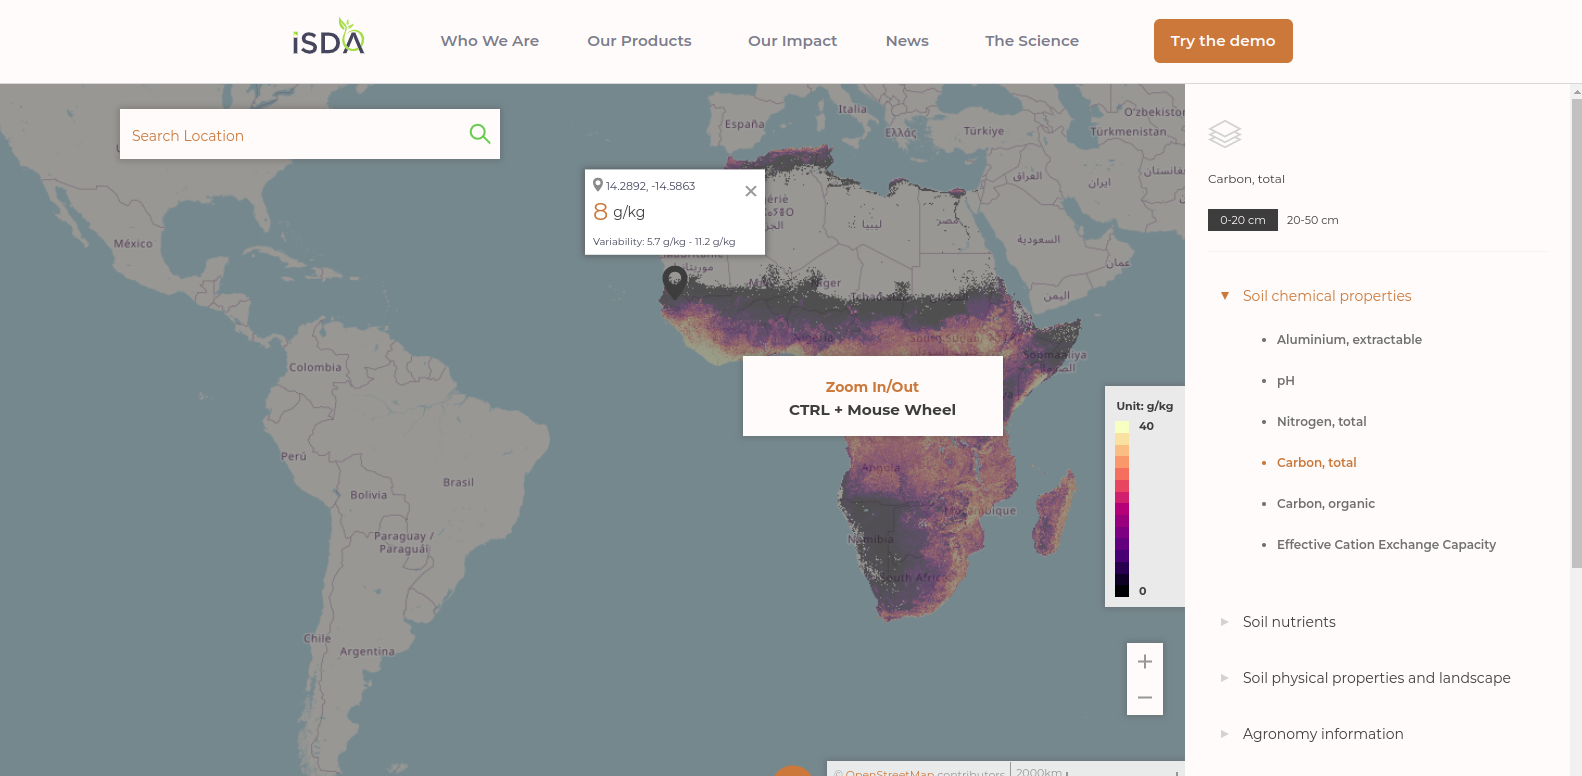
\includegraphics[width=0.9\linewidth]{images/isda.png}
    \caption{ iSDAsoil}
    \label{fig:isda}
\end{figure}

\subsection{SoilGrids}
SoilGrids \cite{soilgrids} (ISRIC) produit des cartes mondiales du SOC à des résolutions typiques de 250 m à 1 km, basées sur des profils harmonisés et des covariables multiples. Si ces produits constituent une référence internationale, leur manque de finesse locale limite leur applicabilité dans les contextes sahéliens, où l’hétérogénéité spatiale est forte.
\begin{figure}[h]
    \centering
    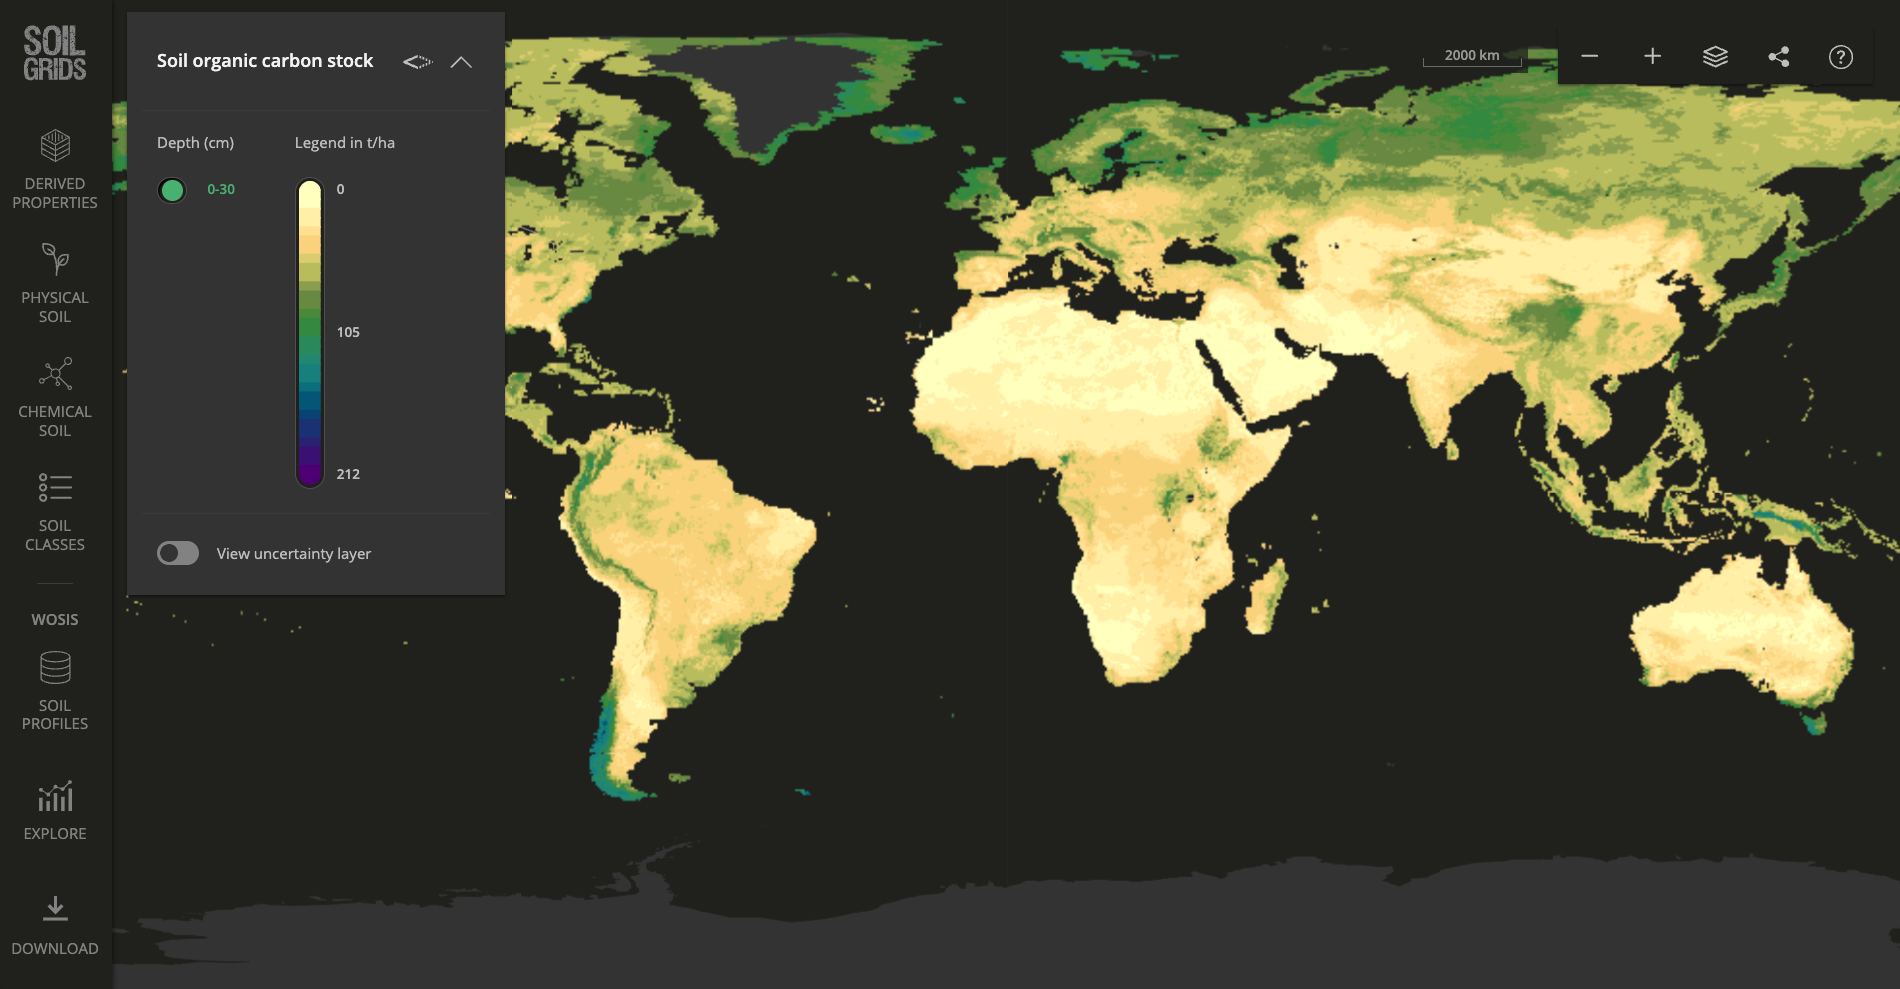
\includegraphics[width=0.9\linewidth]{images/soilgris.png}
    \caption{SoilGrids}
    \label{fig:soilgris}
\end{figure}
\section{Approches de cartographie pédologique}
\subsection{Géostatistique}
La géostatistique \cite{cressie_geostatistics_1989} (variogramme, krigeage) reste une méthode classique pour interpoler le SOC à partir de données ponctuelles. Elle est efficace dans des contextes où la densité d’échantillonnage est élevée, mais sa performance chute lorsque les données sont peu nombreuses ou hétérogènes.
\subsection{Apprentissage automatique}
Les modèles d’apprentissage supervisé (forêts aléatoires, boosting, réseaux de neurones) exploitent \cite{liu_transfer_2018,dong_prediction_2024} la relation entre SOC et covariables optiques, topographiques ou climatiques. Contrairement à la géostatistique, ils capturent mieux les relations non linéaires et s’adaptent à la complexité des interactions sol-végétation-climat. Des approches d’assemblage (stacking) renforcent encore la généralisabilité.
\section{Protocoles d’évaluation et métriques}

La validation est un enjeu crucial\cite{roberts_cross-validation_2017}. Les validations aléatoires surestiment souvent les performances en raison de fuites spatiales. Pour y remédier, des schémas plus rigoureux (ex. GroupKFold par site/profil) sont utilisés, garantissant une séparation stricte des données. Les métriques standards incluent le R²et le RMSE , exprimés en g/kg.
\section{Incertitude et interprétabilité}
La cartographie du SOC ne peut se limiter à une prédiction ponctuelle : il est essentiel de fournir une mesure d’incertitude\cite{vaysse_using_2017}. Celle-ci peut être estimée par :
\begin{itemize}
  \item des ensembles et bootstrap (dispersion inter-modèles),
  \item le Monte Carlo Dropout pour les réseaux de neurones,
  \item l’analyse des résidus et de l’importance des variables, afin d’identifier les zones sous-contraintes en données.
\end{itemize}
\section{Travaux de Thiam (2022–2023)}

En 2022, Thiam a mené une étude sur le même sujet \cite{Thiam2023}.

\subsection{ géostatistique vs apprentissage automatique}
Les travaux de Thiam  comparent des interpolateurs géostatistiques (krigeage) et des modèles de machine learning (forêts et boosting) sur \( \approx 3\,600 \) entrées (\( \approx 1\,800 \) profils) pour deux horizons (0–10 cm et 10–30 cm). Les modèles de machine learning surpassent globalement le krigeage, surtout en 0–10 cm. La précision diminue en 10–30 cm, cohérente avec la moindre sensibilité des capteurs optiques aux couches profondes. Les métriques doivent être rapportées avec unités (g/kg) pour assurer la comparabilité.
\begin{figure}[h]
    \centering
    \begin{subfigure}{0.48\textwidth}
        \centering
        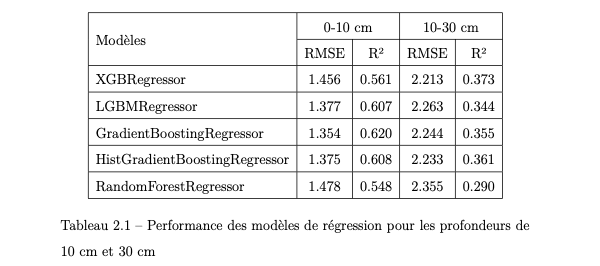
\includegraphics[width=\linewidth]{images/ml.png}
        % \caption{Caption for image 1}
        \label{fig:ml}
    \end{subfigure}%
    \hfill
    \begin{subfigure}{0.48\textwidth}
        \centering
        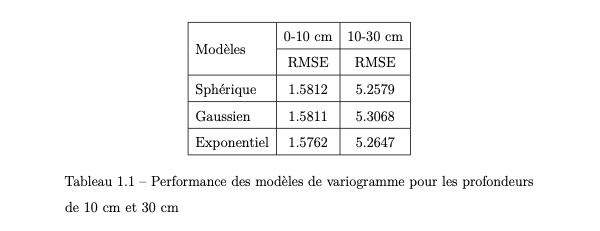
\includegraphics[width=\linewidth]{images/geostatistique.png}
        % \caption{Caption for image 2}
        \label{fig:geostat}
    \end{subfigure}
    \caption{Tiam 2022 : Comparaison entre apprentissage automatique et géostatistique}
    \label{fig:ml_vs_geostat}
\end{figure}
\subsection{Modèles utilisés}
L’étude met en regard des interpolateurs géostatistiques (krigeage ordinaire et variantes) et  des modèles d’apprentissage supervisé . Le protocole retient deux horizons (0–10 et 10–30 cm) et un jeu de \(\sim 3\,600\) entrées correspondant à \(\sim 1\,800\) profils.
\subsection{Résultats}
L’étude de Thiam constitue une référence en contexte sénégalais.
\begin{itemize}
  \item Comparaison géostatistique vs apprentissage automatique : sur $\approx 3\,600$ entrées ($\approx 1\,800$ profils) pour deux horizons ($0$--$10$ cm et $10$--$30$ cm), les modèles d’apprentissage automatique surpassent globalement le krigeage, notamment en surface ($0$--$10$ cm).

\item Limites identifiées :  volume de données encore limité au regard de l’hétérogénéité pédologique,  perte de précision marquée dans la couche 10–30 cm,  absence de cartographie explicite de l’incertitude.
\end{itemize}
Ces résultats confirment la pertinence du machine learning mais soulignent la nécessité de protocoles plus stricts et de l’intégration de nouvelles sources de données.

\begin{figure}[h]
    \centering
    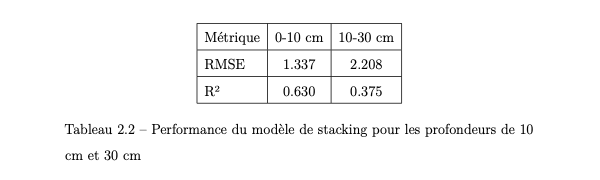
\includegraphics[width=0.9\linewidth]{images/stacking.png}
    \caption{Résultats de Thiam 2022 }
    \label{fig:thiam_results}
\end{figure}


\section{Synthèse et lacunes}
La littérature récente met en évidence :
\begin{itemize}
  \item la puissance des approches d’apprentissage automatique pour améliorer la précision des cartes de SOC,
  \item la nécessité de combiner données locales et globales pour réduire les biais,
  \item l’importance d’intégrer validation spatiale et incertitude pour garantir la robustesse,
  \item la difficulté persistante de prédire les couches profondes (10–30 cm) avec l’optique seule.
\end{itemize}
Ces constats ouvrent la voie à des pipelines reproductibles et enrichis, combinant bases locales (IRD), données satellitaires récentes (Sentinel-2, Landsat-8), et outils de déploiement applicatif.
\\
\newline
C’est dans ce cadre que s’inscrit le présent travail, qui vise à dépasser ces limites en développant un pipeline robuste, intégrant incertitude et reproductibilité, et en proposant une application opérationnelle adaptée au contexte sénégalais.

% ===================== Chapitre 3 =====================
\chapter{Cadre du stage}

\section{Laboratoire d’accueil et encadrement}
Le stage s’est déroulé au sein de l’UMMISCO Sénégal \cite{org-ummisco-2025} (Unité Mixte Internationale de Modélisation Mathématique et Informatique des Systèmes Complexes), basé à l’Université Cheikh Anta Diop (UCAD II) de Dakar.
\\
\newline
UMMISCO est une structure pluridisciplinaire qui associe mathématiques appliquées, informatique et sciences environnementales pour répondre à des enjeux de développement durable. Ses axes de recherche incluent la télédétection, l’intelligence artificielle et la modélisation des écosystèmes complexes.\\
\newline
L’unité fonctionne dans un cadre de coopération internationale, en lien étroit avec l’IRD \cite{org-ird-2025} (Institut de Recherche pour le Développement).
\\
\newline
L’encadrement scientifique a été assuré par des chercheurs spécialisés en pédologie, télédétection et apprentissage automatique. Des réunions hebdomadaires de suivi ont permis d’orienter les choix méthodologiques, de garantir la cohérence avec les objectifs du projet SLAM-B \cite{org-slam-b-2025}, et d’assurer un équilibre entre production scientifique et mise en œuvre applicative.

\newpage

\section{Ferlo-Sine}
Ce stage s’inscrit dans le cadre du projet SLAM-B (Soil Land and Agroecosystem Management in the Ferlo Basin), qui vise à développer des outils innovants pour la gestion durable des terres dans la région du Ferlo.
\newline
Au sein de SLAM-B, le Scenario Lab Ferlo-Sine joue un rôle central. Il constitue un espace collaboratif où chercheurs, institutions locales et décideurs co-construisent des approches de suivi environnemental et socio-économique. L’accent est mis sur :
\begin{itemize}
  \item l’intégration de données de télédétection et de terrain,

\item la simulation des dynamiques agro-écologiques,

\item et le développement d’outils d’aide à la décision pour la gestion des ressources naturelles.
\end{itemize}
Le présent travail s’inscrit directement dans ces objectifs, en proposant un pipeline de prédiction et de cartographie du SOC, assorti d’une application interactive.

\begin{figure}[h]
    \centering
    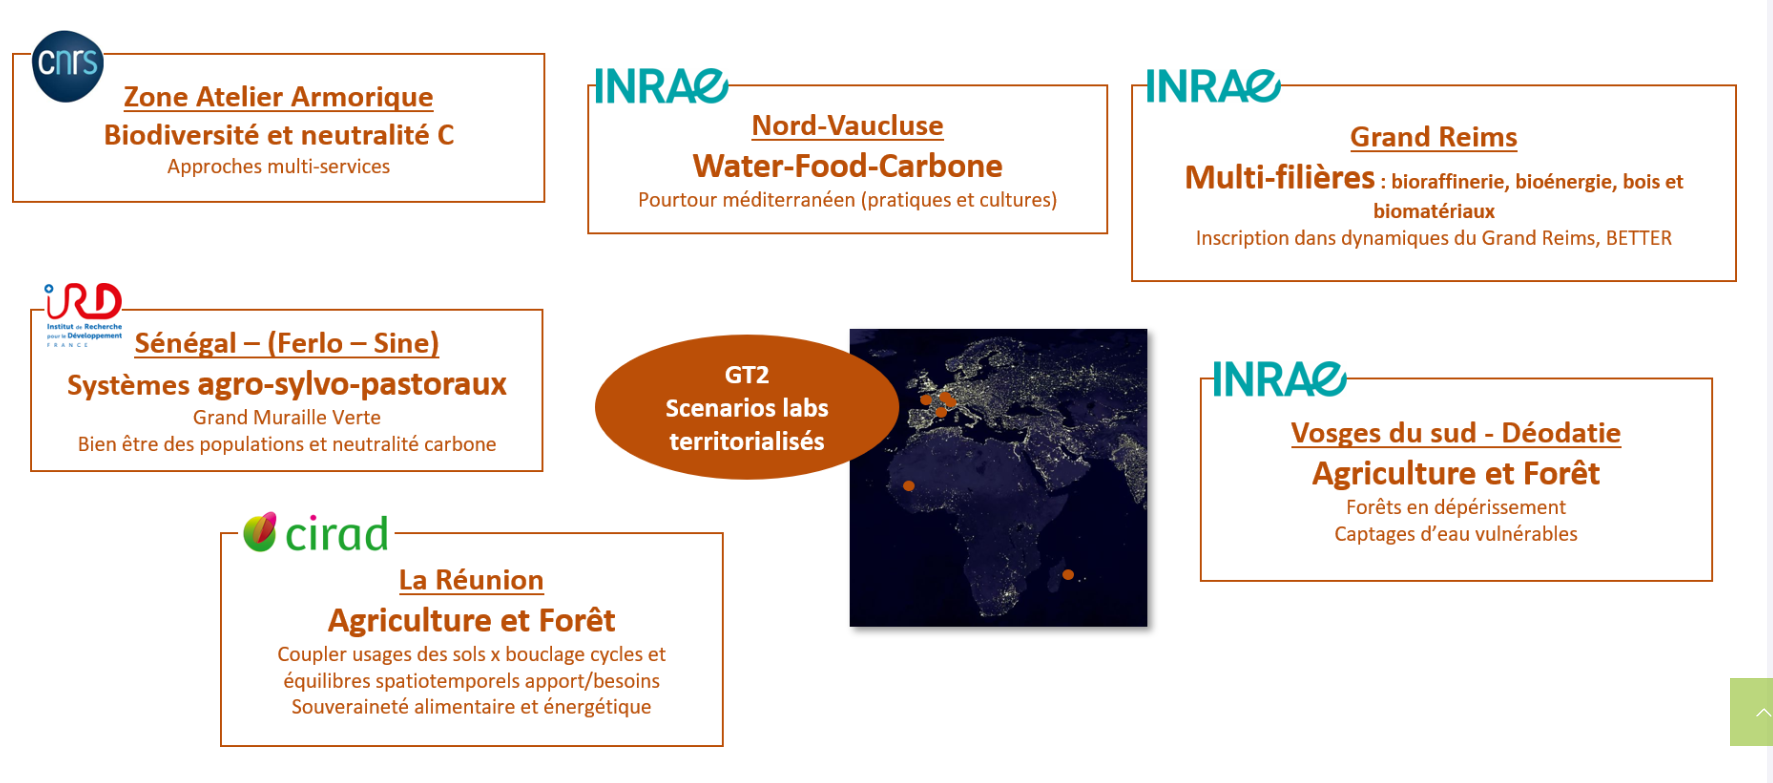
\includegraphics[width=0.7\linewidth]{images/ferlo_sine.png}
    \caption{Ferlo-Sine}
    \label{fig:ferlo_sine}
\end{figure}

\newpage
\section{Zone d’étude : Bary, Diohine/Sassem et Sop}
Trois villages du centre du Sénégal ont été retenus comme sites pilotes :
\begin{figure}[h]
    \centering
    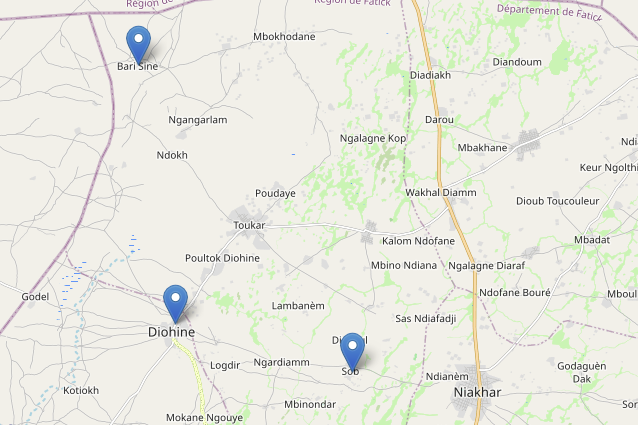
\includegraphics[width=0.5\linewidth]{images/bary_sop_dohien_1.png}
    \caption{Zone d'étude}
    \label{fig:zone_etude}
\end{figure}

Ces trois villages offrent une représentativité intéressante des contextes pédologiques et agroécologiques du bassin arachidier. Leur sélection permet d’évaluer la généralisabilité des modèles de prédiction du SOC dans des environnements variés.

\section{Objectifs opérationnels et jalons}
Le stage avait pour objectif opérationnel la mise en place d’un pipeline complet de prédiction du SOC, depuis la collecte des données jusqu’au déploiement applicatif. Les jalons principaux étaient :
\begin{enumerate}
  \item \textbf{Revue bibliographique et cadrage scientifique} (avril–mai) :analyse des enjeux, méthodologies existantes et identification des lacunes.
  \item \textbf{Collecte et harmonisation des données} (mai–juin) : intégration des profils pédologiques (AfSP, IRD, WoSIS), préparation des images Sentinel-2 et Landsat-8, construction des covariables dérivées.
  \item \textbf{Modélisation et évaluation} (juin–juillet) : entraînement des modèles (forêts aléatoires, boosting, MLP), validation spatiale stricte, analyse des performances et incertitudes.
  \item \textbf{Déploiement applicatif} (juillet–août) : développement d’une API /predict et d’une interface cartographique interactive (Django + PostGIS).
  \item \textbf{Rédaction du mémoire et restitution} (août) : synthèse scientifique, analyse critique, discussion des perspectives.
\end{enumerate}
Cette planification a permis de garantir un équilibre entre recherche et application, avec un produit final à la fois scientifique (pipeline reproductible, résultats chiffrés) et pratique (application opérationnelle).
\begin{figure}[h]
  
\begin{tikzpicture}[
    task/.style={rectangle, draw=blue!60, fill=blue!5, thick, minimum width=3cm, minimum height=1cm},
    milestone/.style={circle, draw=red!60, fill=red!5, thick, minimum size=1cm},
    month/.style={rectangle, draw=black!60, fill=black!20, thick, minimum width=2cm, minimum height=1cm},
    timespan/.style={rectangle, draw=green!60, fill=green!5, thick, minimum width=2cm, minimum height=0.6cm}
]

% Titre
\node[font=\Huge\bfseries] at (6, 9) {Planification de Projet};



% Mois
\node[month] (avr) at (1.5, 7) {Avril};
\node[month, right=0 of avr] (mai) {Mai};
\node[month, right=0 of mai] (jui) {Juin};
\node[month, right=0 of jui] (jul) {Juillet};
\node[month, right=0 of jul] (aou) {Août};
\node[month, right=0 of aou] (sep) {Septembre};

% Tâches
\node[task] (biblio) at (-1.5, 4.5) {Revue bibliographique};
\node[task] (collecte) at (-1.5, 3) {Collecte et pré-traitement};
\node[task] (modele) at (-1.5, 1.5) {Entraînement du modèle};
\node[task] (deploy) at (-1.5, 0) {Développement-Déploiement Web};
\node[task] (rapport) at (-1.5, -1.5) {Rédaction du rapport};

% Barres de progression
\draw[line width=8mm, green!50] (1.5, 4.5) -- (4.5, 4.5);
\draw[line width=8mm, green!50] (3, 3) -- (7.5, 3);
\draw[line width=8mm, green!50] (4.5, 1.5) -- (10.5, 1.5);
\draw[line width=8mm, green!50] (5.5, 0) -- (11.5, 0);
\draw[line width=8mm, green!50] (3.5, -1.5) -- (11.5, -1.5);

% Jalons
% \node[milestone] (milestone1) at (12, -1.5) {};

% Lignes de repère
\foreach \x in {1.5, 3.5, 5.5, 7.5, 9.5, 11.5} {
    \draw[dashed, gray] (\x, 5.5) -- (\x, -2.5);
}

% Dates
\node[anchor=north] at (1.5, 5.5) {15/04};
\node[anchor=north] at (3.5, 5.5) {15/05};
\node[anchor=north] at (5.5, 5.5) {15/06};
\node[anchor=north] at (7.5, 5.5) {15/07};
\node[anchor=north] at (9.5, 5.5) {15/08};
\node[anchor=north] at (11.5, 5.5) {15/09};

% Timeline
\draw[->, thick] (1, 5.5) -- (12.5, 5.5);

\end{tikzpicture}
\end{figure}

% ===================== Chapitre 4 =====================
\chapter{Données et outils}

\section{Sources et caractéristiques des données}
La prédiction du stock de carbone organique du sol (SOC) repose sur la combinaison de données pédologiques de référence et de covariables satellitaires et environnementales.
\subsection{Profils AfSP }
La base Africa Soil Profiles \cite{afsp} (AfSP) constitue une ressource continentale de référence. Elle regroupe 18 533 profils pédologiques collectés à travers l’Afrique entre 1938 et 2011, chacun comprenant jusqu’à quatre couches de profondeur.
\begin{itemize}
  \item Avantage : taille du jeu de données, diversité spatiale et richesse des attributs physico-chimiques.

\item Limite : hétérogénéité temporelle (décalage par rapport aux satellites récents) et variabilité dans les méthodes de mesure.
\end{itemize}
Seuls les horizons 0–10 cm et 10–30 cm ont été retenus pour rester cohérents avec les profils IRD et WoSIS.
\begin{figure}[h]
    \centering
    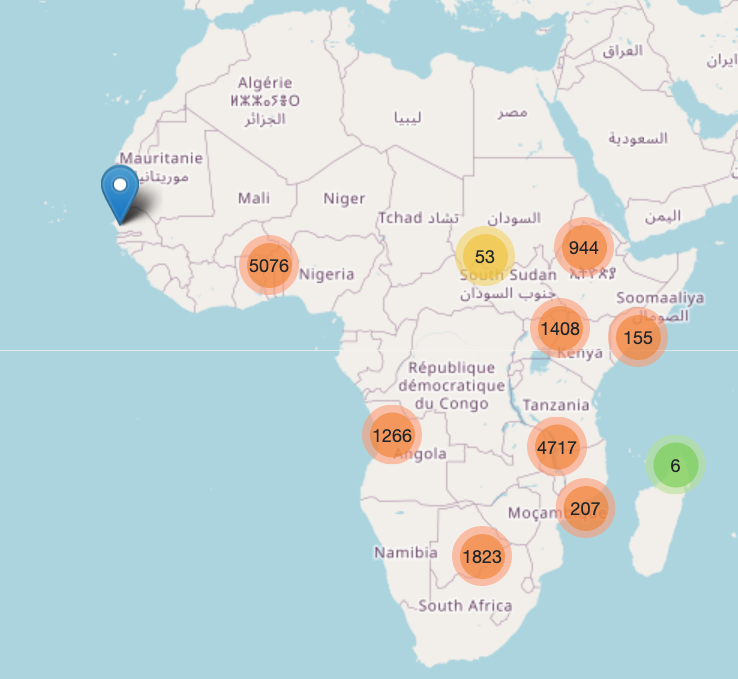
\includegraphics[width=0.3\textwidth]{images/afsp.png}
    \caption{Profils AfSP}
    \label{fig:afsp}
\end{figure}
\subsection{Données locales de l’IRD}
L’\textbf{Institut de Recherche pour le Développement (IRD)} a fourni un jeu de données local spécifiquement centré sur le Sénégal (Ferlo-Sine).
\begin{itemize}
  \item Taille : environ 1 800 profils (deux horizons : 0–10 cm et 10–30 cm).

\item Période d’échantillonnage : 2016–2017, contemporaine des séries Sentinel-2 et Landsat-8.

\item Avantage : synchronisation temporelle avec les satellites, permettant une calibration robuste.

\item Limite : couverture restreinte à quelques villages pilotes (Bary, Diohine/Sassem, Sop), ce qui limite la généralisabilité directe.
\end{itemize}
Ces données constituent la base de validation principale du pipeline développé.
\begin{figure}[h]
    \centering
    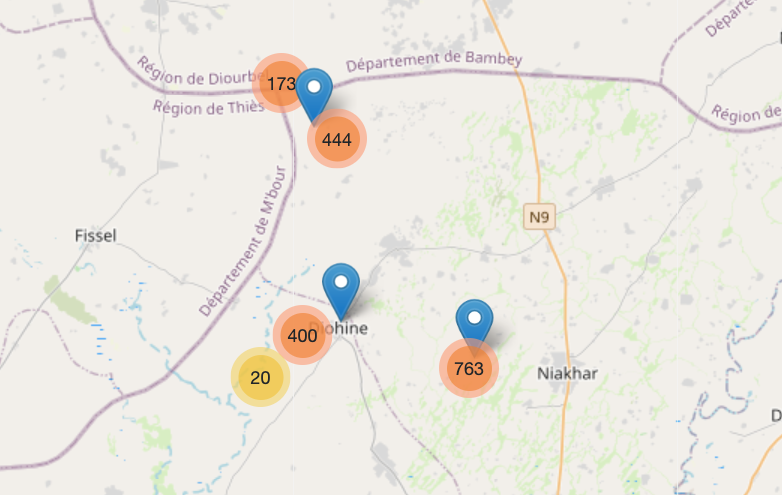
\includegraphics[width=0.9\linewidth]{images/zone.png}
    \caption{Zone d'étude}
    \label{fig:zone}
\end{figure}
\subsection{Profils WoSIS}
La base \textbf{WoSIS (World Soil Information Service)} \cite{wosis} compilée par l’ISRIC, rassemble plus de 196 297 profils pédologiques mondiaux.
\begin{itemize}
  \item Caractéristiques : nombre de couches variable selon les profils ; période de collecte souvent inconnue ou hétérogène.

\item Avantage : dimension internationale et homogénéisation des profils, utile pour situer les valeurs locales dans un cadre global.

\item Limite : incohérences dans les profondeurs et manque d’informations temporelles.

\end{itemize}
Dans ce travail, WoSIS est mobilisé comme cadre de comparaison global et pour enrichir l’entraînement des modèles.
\begin{figure}[h]
    \centering
    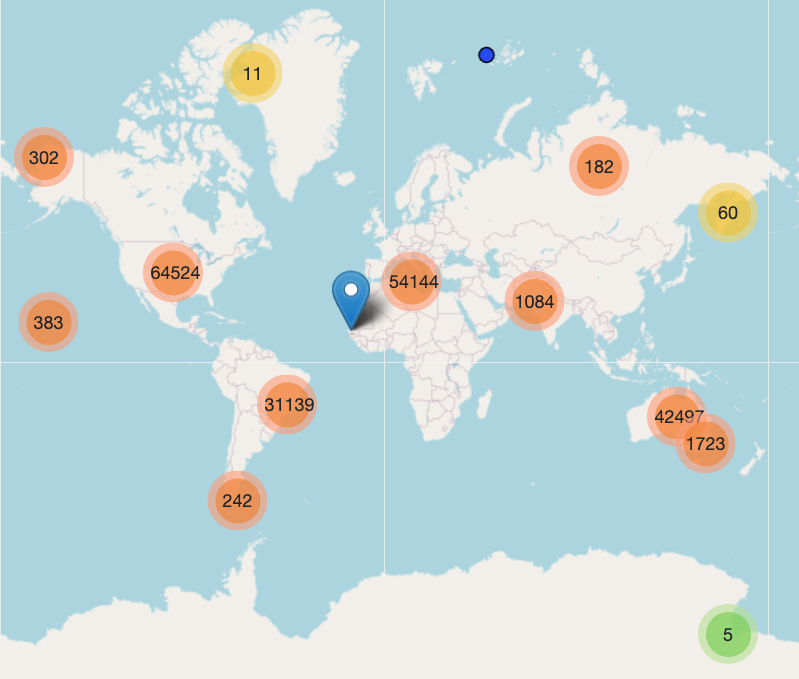
\includegraphics[width=0.5\linewidth]{images/wosis.png}
    \caption{Profils WoSIS}
    \label{fig:wosis}
\end{figure}
\subsection{Imagerie Sentinel-2 et Landsat-8}
L’imagerie satellitaire constitue la principale source de covariables spatiales :
\begin{itemize}
  \item \textbf{Sentinel-2 \cite{sentinel2} (MSI)} : données multispectrales à 10--20 m de résolution spatiale, couvrant la période 2015--2025.
  \item \textbf{Landsat-8 \cite{landsat8} (OLI/TIRS)} : données multispectrales à 30 m, disponibles depuis 2013, permettant d’allonger la série temporelle.
\end{itemize}
Ces deux familles de capteurs offrent une complémentarité : haute résolution spatiale pour Sentinel-2 et profondeur temporelle pour Landsat-8.

\subsection{Variables dérivées (indices spectraux, topographie, sols globaux)}
À partir des images satellites et de bases complémentaires, plusieurs covariables ont été construites :
\begin{itemize}
  \item \textbf{Indices spectraux} : NDVI (végétation), NDWI (humidité), BSI (sols nus), CI-Green (chlorophylle).
  \item \textbf{Variables topographiques} : altitude, pente, exposition issues de modèles numériques de terrain (SRTM, Copernicus DEM).
\end{itemize}

\section{Préparation et qualité des données}

\subsection{Contrôles et nettoyage}
Un ensemble de contrôles a été mis en place pour garantir la fiabilité des données :
\begin{itemize}
  \item Détection et suppression des doublons ou valeurs aberrantes dans les profils.
  \item Masquage des nuages dans Sentinel-2 et Landsat-8.
  \item Vérification de la cohérence .
\end{itemize}

\subsection{Harmonisation spatiale et temporelle}
Les données ont été harmonisées afin de permettre leur intégration dans un même pipeline :
\begin{itemize}
  \item Projection dans un système de coordonnées commun (WGS84 / UTM).
  \item Normalisation des profondeurs en 0--10 cm et 0--30 cm pour assurer une cohérence avec les cibles retenues.
\end{itemize}






% ===================== Chapitre 5 =====================
\chapter{Méthodologie}

\section{Pipeline de collecte et préparation des données}
Le pipeline de données a été construit afin de relier les observations pédologiques ponctuelles avec les variables de télédétection et environnementales. L’ensemble du processus a été automatisé via \textbf{Google Earth Engine (GEE)} et complété par des scripts Python. Les principales étapes sont :
\begin{enumerate}
\item \textbf{Filtrage spatial (zones d’intérêt) }: Bary, Diohine/Sassem, Sop),
\item \textbf{Filtrage temporel} (2013–2025 pour Landsat-8, 2015–2025 pour Sentinel-2),
\item \textbf{Sélection des capteurs et période} : Sentinel-2 (2015–2025) et Landsat-8 (2013–2025).
\item \textbf{Nettoyage : Filtres de qualité} : masques de nuages (Sentinel-2 QA60).
\item \textbf{Agrégation trimestrielle (médiane)} : médianes trimestrielles pour réduire le bruit et capturer la saisonnalité.

\item \textbf{Extraction ponctuelle pour chaque profil pédologique},
\item \textbf{Extraction des variables dérivées} : indices spectraux (NDVI, NDWI, BSI, CI-Green), polarisation radar (VV, VH, ratio), variables topographiques et pédologiques.
\item \textbf{Harmonisation et intégration} : reprojection sur une grille commune et intégration dans PostGIS.


\end{enumerate}

Le pipeline s’appuie uniquement sur l’optique (Sentinel-2 L2A, Landsat-8 OLI/TIRS). Après filtrage qualité (masques nuages) et agrégation en composites trimestriels, nous extrayons NDVI, NDWI, BSI, CI-Green ainsi que des covariables topographiques (MNT, pente, exposition) et pédologiques globales. Ces variables alimentent des modèles tabulaires (RF, boosting) et un MLP PyTorch, avec normalisation adéquate et GroupKFold par site. 

\begin{figure}[h]

\begin{tikzpicture}[
  node distance=5mm and 5mm,
  box/.style={rectangle, draw, rounded corners, align=right, minimum width=10mm, minimum height=8mm},
  arrow/.style={-{Latex[length=2mm]}}]

\node[box] (sites) {Coordonées profils  \\(1800 points)};
\node[box, right=of sites] (sat) {API GEE \\Sentinel-2,Landsat-8};
% \node[box, below=of s2] (s1) {Sentinel-1\\GRD VV/VH};
\node[box, right=of sat] (bands) {Bandes spectral };
\node[box, right=of bands] (feats) {Indices/Stats\\NDVI,EVI,NDWI,\\BSI,RECI, VV/VH};


\draw[arrow] (sites) -- (sat);
\draw[arrow] (sat) -- (bands);
\draw[arrow] (bands) -- (feats);

\end{tikzpicture}

\caption{ pipeline de collecte des données satellites.}
\end{figure}



\subsection{Optimisation et réglage des modèles}
Une optimisation systématique des hyperparamètres a été réalisée :
\begin{itemize}
\item Recherche en grille et optimisation bayésienne (Optuna).
\item Paramètres explorés : profondeur maximale, nombre d’arbres, taux d’apprentissage, régularisation.
\item Validation croisée imbriquée pour sélectionner les configurations robustes.
\end{itemize}

\section{Multi-Layer Perceptron}
Un modèle avancé a été implémenté sous PyTorch afin d’exploiter la capacité des réseaux de neurones à modéliser des relations complexes.
\begin{itemize}
\item \textbf{Architecture} : couches denses (256–128–64 neurones), activation ReLU, dropout (0.2–0.3).
\item \textbf{Normalisation} : standardisation des variables continues et encodage des variables catégorielles.
\item \textbf{Fonction de perte} : erreur quadratique moyenne (MSE).
\item \textbf{Stratégie OOF (Out-Of-Fold)} : entraînement croisé avec sauvegarde des prédictions par pli.
\end{itemize}

% code architecture MLP 

\section{Quantification et cartographie de l’incertitude}
L’incertitude des prédictions a été intégrée pour renforcer la valeur décisionnelle des cartes produites :
\begin{itemize}
\item \textbf{Ensembles et bootstrap} : variance des prédictions entre modèles.
\item \textbf{Dropout bayésien} : approximation par Monte Carlo Dropout.
\item \textbf{Cartes d’écart-type} : représentation spatiale de la dispersion des prédictions.
\item \textbf{Intervalles de confiance (90\%)} : bornes inférieure et supérieure des prédictions de SOC.
\end{itemize}

\section{Limites méthodologiques et ajustements}

Une approche initiale consistait à entraîner un modèle générique sur la base AfSP (18 533 profils, 4 couches, 1938–2011), puis à effectuer un fine-tuning local sur les données IRD.

Cependant, le décalage temporel entre AfSP et les satellites récents (Sentinel-2 à partir de 2015) a limité la transférabilité directe. Les ajustements ont donc consisté à :

privilégier les données synchronisées temporellement (IRD 2016–2017),

restreindre les horizons aux couches superficielles (0–10 cm, 10–30 cm),

intégrer les bases WoSIS et SoilGrids comme complément de calibration.

\section{Innovations méthodologiques}
Par rapport aux travaux antérieurs (ex. Thiam, 2022–2023), ce mémoire introduit plusieurs innovations :
\begin{itemize}
  \item Validation Leave-Area-Out (LAO)

\item Chaque village (Bary, Diohine/Sassem, Sop) est exclu à tour de rôle du jeu d’entraînement et utilisé comme zone de test indépendante.

\item Cela permet d’évaluer la généralisabilité spatiale des modèles et de détecter les biais liés à la structure des données.

\item Prédiction hiérarchique SOC10 → SOC30

\item La prédiction du SOC à 10–30 cm intègre comme covariable le SOC prédit en surface (0–10 cm).

\item Ce transfert améliore la stabilité des prédictions dans les couches profondes, moins bien captées par la télédétection optique.

\item Approche par site

\item Des modèles spécifiques ont été calibrés pour chaque village pilote afin de capturer les spécificités locales, avant d’être comparés à un modèle global.
\end{itemize}
Ces innovations renforcent à la fois la robustesse méthodologique et la pertinence opérationnelle du pipeline.
% figure de d'apprentissage  de soc_10 et soc_30 tikz node

\begin{figure}[h]
\centering
\begin{tikzpicture}[node distance=1.5cm and 1.8cm, every node/.style={font=\small}]

\tikzstyle{data} = [rectangle, draw, fill=blue!20, text centered, minimum width=3cm, minimum height=1cm]
\tikzstyle{model} = [rectangle, draw, fill=green!20, text centered, minimum width=3cm, minimum height=1cm]
\tikzstyle{output} = [rectangle, draw, fill=orange!30, text centered, minimum width=4cm, minimum height=1cm]
\tikzstyle{arrow} = [thick, ->, >=Stealth]

% Phase 1
\node[data] (soil) {Profils de sol (Données pédologiques)};
\node[data, right=of soil] (sentinel) {Images satellites (Sentinel-2,Landsat-8)};


% Phase 2
\node[model, at = ($(soil)!0.5!(sentinel)$), below=of soil] (model) {Modèle de prédiction};

% Phase 3
\node[output, below=of model] (output) {Carte SOC (Stock de Carbone dans le Sol)};

% Arrows
\draw[arrow] (soil) -- (model);
\draw[arrow] (sentinel) -- (model);
\draw[arrow] (model) -- (output);


% Labels
\node[above=0.5cm of soil, font=\bfseries] {Phase 1 : Données};
\node[left=0.7cm of model, font=\bfseries] {Phase 2 : Modèle};
\node[below=0.5cm of output, font=\bfseries] {Phase 3 : Résultat};

\end{tikzpicture}
\caption{Écosystème du modèle de prédiction du stock de carbone dans le sol}
\end{figure}

\newpage
\section{Modèles de référence}
Afin d’établir une base comparative solide, plusieurs modèles supervisés ont été entraînés:
\begin{itemize}
\item Régression linéaire régularisée (Ridge, Lasso),
\item Forêts aléatoires (RF),
\item Gradient Boosting (XGB, LightGBM, HistGradientBoosting).
\end{itemize}
\noindent Les validations ont suivi un schéma rigoureux :
\begin{itemize}
\item \textbf{GroupKFold par site} : les profils d’un même village sont exclus du jeu d’apprentissage lorsqu’ils sont utilisés pour le test, afin d’éviter toute fuite spatiale.
\item \textbf{Métriques} : coefficient de détermination (R2), erreur quadratique moyenne (RMSE) .
\end{itemize}
\begin{figure}[h]
\centering
\begin{tikzpicture}[
  node distance=5mm and 5mm,
  box/.style={rectangle, draw, rounded corners, align=right, minimum width=10mm, minimum height=8mm},
  arrow/.style={-{Latex[length=2mm]}}]

\node[draw, minimum width=3cm, minimum height=1cm] (data) {Données satellitaires, pédologiques};

\node[draw, minimum width=3cm, minimum height=1cm, right=0.5cm of data] (Model_10) {Model\_10};

\node[draw,ellipse, minimum width=3cm, minimum height=1cm, right=0.5cm of Model_10] (soc_10) {SOC 0-10 g/kg};
\node[draw, minimum width=3cm, minimum height=1cm, below=0.5cm of Model_10] (Model_30) {Model\_30};
\node[draw, ellipse, minimum width=1cm, minimum height=1cm, below=0.5cm of Model_30] (soc_30) {SOC 10-30 g/kg};


% Arrows
\draw[arrow] (data) -- (Model_10);
\draw[arrow] (Model_10) -- (soc_10);
\draw[arrow] (Model_30) -- (soc_30);
\draw[arrow] (data) |- (Model_30);
\draw[arrow] (soc_10) |- (Model_30);



% node test in bottom-right CORNER of model_30

\end{tikzpicture}
\caption{Apprentissage des modèles pour les couches de SOC 0-10 cm et 10-30 cm}
\end{figure}


% ===================== Chapitre 6 =====================
\chapter{Résultats}

\section{Modèles de référence}
Les modèles de référence incluent plusieurs méthodes d’apprentissage supervisé basées sur des arbres de décision (Random Forest, Gradient Boosting, XGBoost, LightGBM, HistGradientBoosting), ainsi qu’un assemblage par stacking. Les résultats (Tableau 6.1) montrent des performances variables selon la profondeur du sol.
\begin{table}[h]
\centering
\begin{tabular}{l l l l l}
\toprule
\multirow{2}{*}{\textbf{Modèle}} & \multicolumn{2}{l}{\textbf{0-10}} & \multicolumn{2}{l}{\textbf{0-30}} \\
\cmidrule(lr){2-3} \cmidrule(lr){4-5}
& \textbf{R²} & \textbf{RMSE} & \textbf{R²} & \textbf{RMSE} \\
\midrule
LGBMR & 0.63 & 0.97 &0.42 &0.72 \\
GBR & 0.54 & 1.20 & 0.40 &0.75 \\
XGBR & 0.57 & 1.12 & 0.39 &0.76 \\
HistGradientBoosting & 0.65 & 0.90 & 0.43 &0.72 \\
RandomForest & 0.61 & 1.02 & 0.45 &0.70 \\
stacking & 0.57 & 1.05 & 0.41 &0.74 \\

\bottomrule
\end{tabular}
\caption{Résultats des modèles de référence.}
\end{table}

Pour la couche 0–10 cm, les coefficients de détermination (R²) se situent entre 0.54 (Gradient Boosting) et 0.65 (HistGradientBoosting), avec des RMSE compris entre 0.90 et 1.20 g/kg. Ces valeurs indiquent une capacité prédictive correcte, mais encore limitée pour capturer les variations fines du SOC en surface. Parmi ces modèles, HistGradientBoosting apparaît comme le plus performant (R² = 0.65 ; RMSE = 0.90), probablement en raison de sa capacité à gérer les distributions hétérogènes et les relations non linéaires complexes.
\\
\newline
Pour la couche 10–30 cm, les performances sont globalement plus faibles, avec des R² variant de 0.39 (XGBR) à 0.45 (Random Forest). Les RMSE se situent autour de 0.70–0.76 g/kg. Ces résultats confirment que les indices spectraux issus de l’imagerie optique sont moins sensibles aux horizons profonds, ce qui complique la prédiction du SOC à 30 cm. Néanmoins, le Random Forest obtient les meilleurs résultats relatifs en profondeur (R² = 0.45 ; RMSE = 0.70), traduisant une meilleure robustesse aux données bruitées.
\\
\newline
L’assemblage par stacking, censé combiner les forces des différents modèles, n’apporte pas d’amélioration significative dans ce cas (R² = 0.57 et 0.41 pour 0–10 cm et 10–30 cm respectivement). Cela peut s’expliquer par la forte corrélation entre les modèles de base (tous issus d’arbres de décision), qui limite la complémentarité des prédictions.
\\
\newline
En résumé, les modèles de référence parviennent à capturer une partie de la variabilité du SOC, mais leurs performances demeurent modestes, en particulier pour les couches profondes. Ces résultats justifient l’exploration de modèles plus puissants et flexibles, tels que les réseaux de neurones artificiels, afin de mieux exploiter la richesse des covariables et de dépasser les limites observées.

\section{MLP}

Le réseau de neurones Multi-Layer Perceptron (MLP), implémenté sous PyTorch, a montré des performances nettement supérieures à celles des modèles de référence. Les résultats par profondeur et par site (Tableau 6.2) révèlent plusieurs tendances
% Tableau exemple
\begin{table}[h]
\centering
\caption{Performances par profondeur et site .}
\begin{tabular}{lccc}
\toprule
Profondeur & Site & \Rtwo~(test) & \RMSE~(test) \\
\midrule
10 cm & 0 & 0.78 & 0.55 \\
10 cm & 1 & 0.87 & 0.43 \\
10 cm & 2 & 0.76 & 0.54 \\
10 cm & all & 0.80 & 0.52 \\
\midrule
30 cm & 0 & 0.59 & 0.76 \\
30 cm & 1 & 0.68 & 0.62 \\
30 cm & 2 & 0.62 & 0.60 \\
30 cm & all & 0.65 & 0.66 \\
\bottomrule
\end{tabular}
\end{table}
Pour la couche 0–10 cm, les prédictions atteignent un coefficient de détermination global de R² = 0.80 avec un RMSE de 0.52 g/kg, soit une amélioration notable par rapport aux modèles d’arbres (meilleurs R² $\approx 0.65$ ). Localement, les performances varient légèrement entre villages : Diohine/Sassem obtient les scores les plus élevés (R² = 0.87 ; RMSE = 0.43), tandis que Bary et Sop restent solides (R² entre 0.76 et 0.78). Ces résultats confirment la sensibilité de l’imagerie optique aux couches superficielles et la capacité du MLP à exploiter pleinement les interactions complexes entre indices spectraux et covariables pédologiques.
\\
\newline
Pour la couche 10–30 cm, les performances restent plus modestes mais néanmoins meilleures que celles des modèles de référence : R² global = 0.65 et RMSE = 0.66 g/kg. Les scores varient de 0.59 (Bary) à 0.68 (Diohine/Sassem). Comme attendu, les horizons profonds sont plus difficiles à prédire, la télédétection optique captant surtout les caractéristiques de surface. Toutefois, l’approche hiérarchique (intégration du SOC prédit à 0–10 cm comme covariable pour 10–30 cm) contribue à stabiliser les résultats et limite la dégradation de la performance.




\subsection{Cartographie des prédictions du SOC et analyse des incertitudes}

Les figures ci-dessous présentent les cartes de prédictions du stock de carbone organique du sol (SOC) pour les deux profondeurs étudiées, obtenues après agrégation sur une maille régulière de 250 m.

\subsubsection*{SOC 0--10 cm}
La carte SOC\textsubscript{10} (Fig.~\ref{fig:soc_maps}, gauche) met en évidence une forte hétérogénéité spatiale, avec des valeurs comprises entre 2 et 8 g·kg\(^{-1}\). Plusieurs zones localisées, notamment au centre et au nord de la zone d’étude, présentent des teneurs plus élevées en carbone.  
Cette variabilité est cohérente avec les conditions pédologiques et l’occupation des sols, la couche superficielle étant directement influencée par la végétation, les pratiques agricoles et les apports organiques.  
Le modèle semble donc capturer efficacement les contrastes de surface détectables par les données de télédétection.

\subsubsection*{SOC 0--30 cm}
La carte SOC\textsubscript{30} (Fig.~\ref{fig:soc_maps}, droite) présente une structure spatiale globalement similaire mais avec des valeurs moyennes légèrement plus faibles et une variabilité plus atténuée.  
L’échelle des prédictions s’étend de 2 à 9 g·kg\(^{-1}\), mais la majorité des mailles se situe entre 2 et 6 g·kg\(^{-1}\).  
Cette homogénéisation relative reflète la difficulté à estimer le carbone en profondeur, les signaux satellitaires étant principalement sensibles aux couches superficielles.

\begin{figure}[h!]
    \centering
    \begin{subfigure}[b]{0.48\textwidth}
        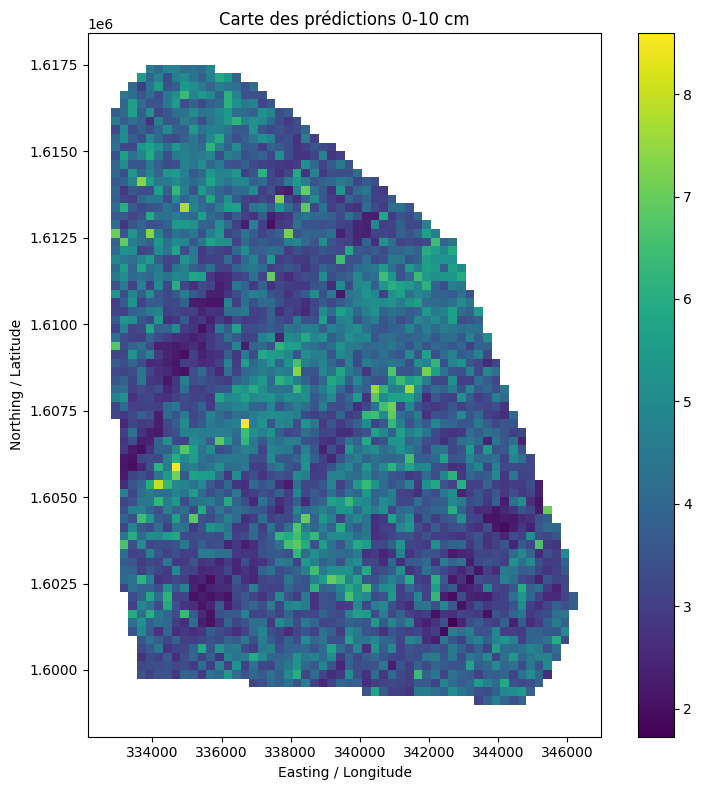
\includegraphics[width=\linewidth]{images/soc10_map.png}
        \caption{Prédictions SOC\textsubscript{10} (0--10 cm)}
    \end{subfigure}
    \hfill
    \begin{subfigure}[b]{0.48\textwidth}
        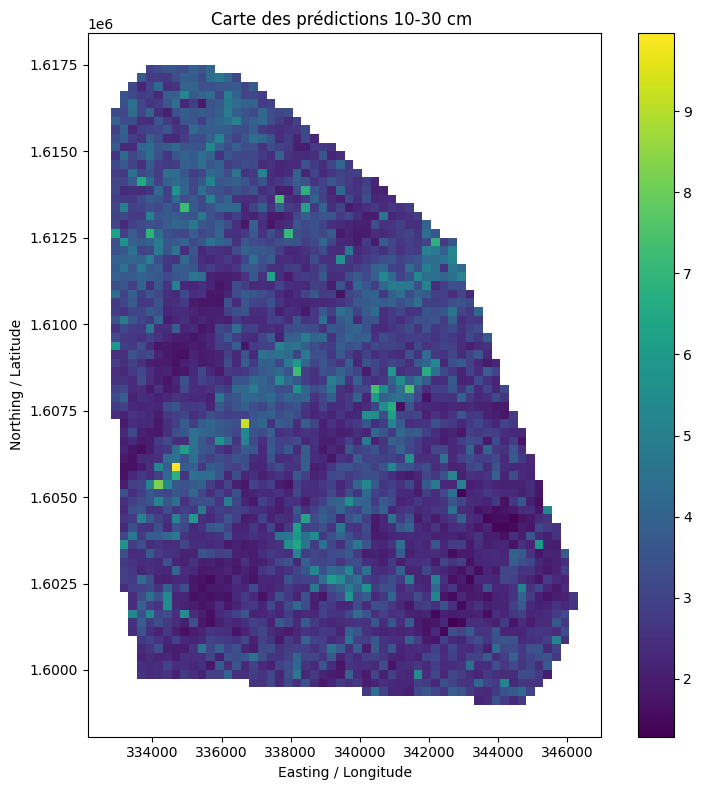
\includegraphics[width=\linewidth]{images/soc30_map.png}
        \caption{Prédictions SOC\textsubscript{30} (0--30 cm)}
    \end{subfigure}
    \caption{Cartes de prédictions du SOC obtenues à partir du modèle sur une maille de 250 m.}
    \label{fig:soc_maps}
\end{figure}

\subsubsection*{Analyse des incertitudes}
Afin d’évaluer la robustesse des prédictions, la distribution des moyennes ($\mu$), des écarts-types ($\sigma$) et de la largeur des intervalles de confiance à 90\% (IC90) a été examinée pour chaque profondeur (Fig.~\ref{fig:uncertainty_hist}).

Pour le SOC\textsubscript{10}, les prédictions présentent des incertitudes faibles, avec $\sigma$ centré autour de 0.15--0.20 et des IC90 étroits ($\approx$ 0.4--0.6).  
En revanche, pour le SOC\textsubscript{30}, les incertitudes sont plus marquées : $\sigma$ atteint souvent 0.20--0.25 et les IC90 sont en moyenne deux fois plus larges ($\approx$ 0.7--1.0).  
Cela confirme que les estimations en surface sont plus fiables, tandis que celles en profondeur doivent être interprétées avec davantage de prudence.

\begin{figure}[h!]
    \centering
    \begin{subfigure}[b]{0.95\textwidth}
        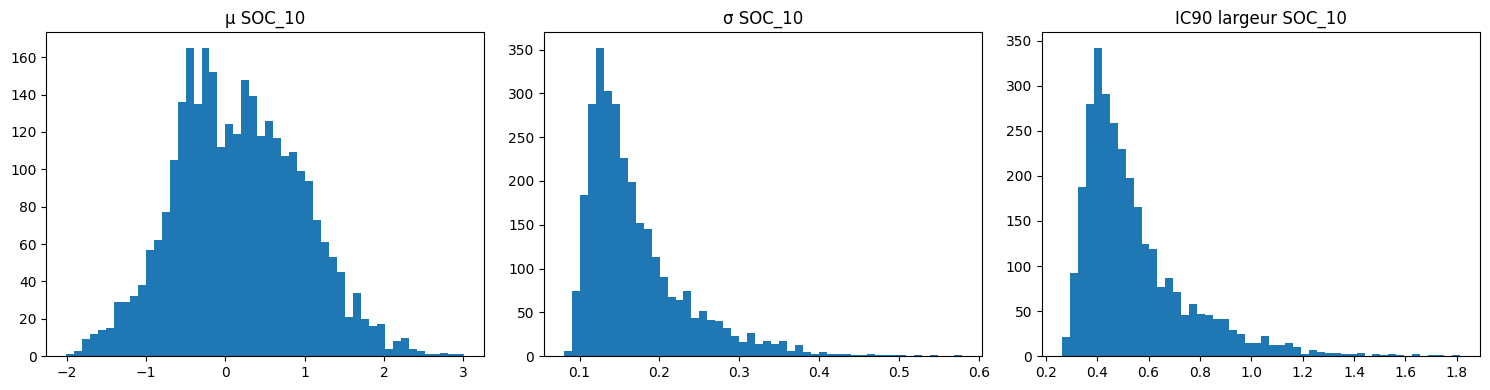
\includegraphics[width=\linewidth]{images/soc10_uncertainty.png}
        \caption{Distribution des incertitudes pour SOC\textsubscript{10} (0--10 cm)}
    \end{subfigure}
    \vskip 0.5cm
    \begin{subfigure}[b]{0.95\textwidth}
        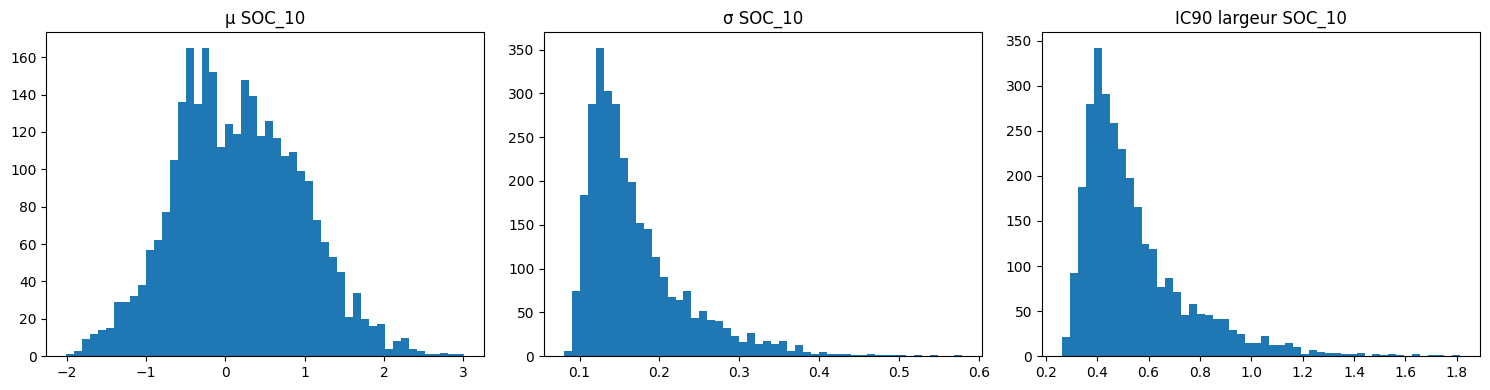
\includegraphics[width=\linewidth]{images/soc30_uncertainty.png}
        \caption{Distribution des incertitudes pour SOC\textsubscript{30} (0--30 cm)}
    \end{subfigure}
    \caption{Histogrammes des moyennes ($\mu$), des écarts-types ($\sigma$) et des largeurs d’IC90 des prédictions SOC.}
    \label{fig:uncertainty_hist}
\end{figure}




\section{Analyse comparative des modèles}

\begin{table}[h]
\centering
\begin{tabular}{l l l l l}
\toprule
\multirow{2}{*}{\textbf{Modèle}} & \multicolumn{2}{l}{\textbf{0-10}} & \multicolumn{2}{l}{\textbf{0-30}} \\
\cmidrule(lr){2-3} \cmidrule(lr){4-5}
& \textbf{R²} & \textbf{RMSE} & \textbf{R²} & \textbf{RMSE} \\
\midrule
LGBMR & 0.63 & 0.97 &0.42 &0.72 \\
GBR & 0.54 & 1.20 & 0.40 &0.75 \\
XGBR & 0.57 & 1.12 & 0.39 &0.76 \\
HistGradientBoosting & 0.65 & 0.90 & 0.43 &0.72 \\
RandomForest & 0.61 & 1.02 & 0.45 &0.70 \\
stacking & 0.57 & 1.05 & 0.41 &0.74 \\
PyTorch MLP  & 0.80 & 0.52 & 0.65 &0.66 \\
\bottomrule
\end{tabular}
\caption{Comparaison des performances entre les modèles.}
\end{table}

% \subsection{Points forts et limites}

% \textbf{Modèles de référence :}
% \begin{itemize}
%   \item Avantage :.
%   \item Limite :.
% \end{itemize}

% \textbf{MLP :}
% \begin{itemize}
%   \item Avantages :.
%   \item Limites : .
% \end{itemize}

\section{Conclusion}

La comparaison des modèles montre que le MLP sous PyTorch surpasse nettement les modèles de référence, avec des R² de 0.80 (0–10 cm) et 0.65 (10–30 cm), et des RMSE respectifs de 0.52 g/kg et 0.66 g/kg.
Les erreurs sont plus faibles en surface (RMSE $\approx$ 0.52 g/kg) qu’en profondeur (RMSE $\approx$ 0.66 g/kg).
\\
Les zones à faible densité d’échantillonnage présentent des erreurs plus élevées, confirmant l’importance de la répartition spatiale des profils.
\\
Les valeurs extrêmes de SOC (très faibles ou très élevées) sont parfois mal prédites, reflétant une limite d’extrapolation des modèles.\\
Les modèles à base d’arbres ont tendance à sous-estimer les fortes valeurs de SOC, du fait de leur effet régularisateur.

\bigskip

L’analyse des erreurs résiduelles met en évidence plusieurs éléments clés :

\begin{itemize}
    \item Les erreurs sont globalement plus faibles pour la couche 0--10 cm (\textit{RMSE} = 0{,}52) que pour la couche 10--30 cm (\textit{RMSE} = 0{,}66), ce qui reflète la plus grande sensibilité des capteurs optiques et radar à la surface du sol.
    
    \item Les zones à faible densité d’échantillonnage présentent des erreurs plus élevées, ce qui confirme un biais spatial lié à l’inégale répartition des profils pédologiques.

    \item Certains profils avec des valeurs extrêmes de SOC (très faibles ou très élevées) sont mal prédits par les modèles, suggérant une capacité d’extrapolation limitée au-delà du domaine d’apprentissage.

    \item Les modèles basés sur les arbres (RF, XGB, LGBM) ont tendance à sous-estimer les valeurs très élevées de SOC, en raison de leur effet régularisateur.

\end{itemize}


Ces résultats soulignent la pertinence des estimations en surface pour la cartographie opérationnelle du SOC et la nécessité de compléter les prédictions en profondeur par des données pédologiques locales pour fiabiliser les estimations.
web développée, permettant une consultation interactive et une interrogation par coordonnées GPS.
% \begin{figure}[h]\centering\includegraphics[width=.8\linewidth]{figures/carte_soc10.png}\caption{Carte SOC 10 cm.}\end{figure}

% ===================== Chapitre 7 =====================



\chapter{Déploiement applicatif}


\begin{figure}[h]
  \centering
  \begin{subfigure}{0.48\textwidth}
      \centering
      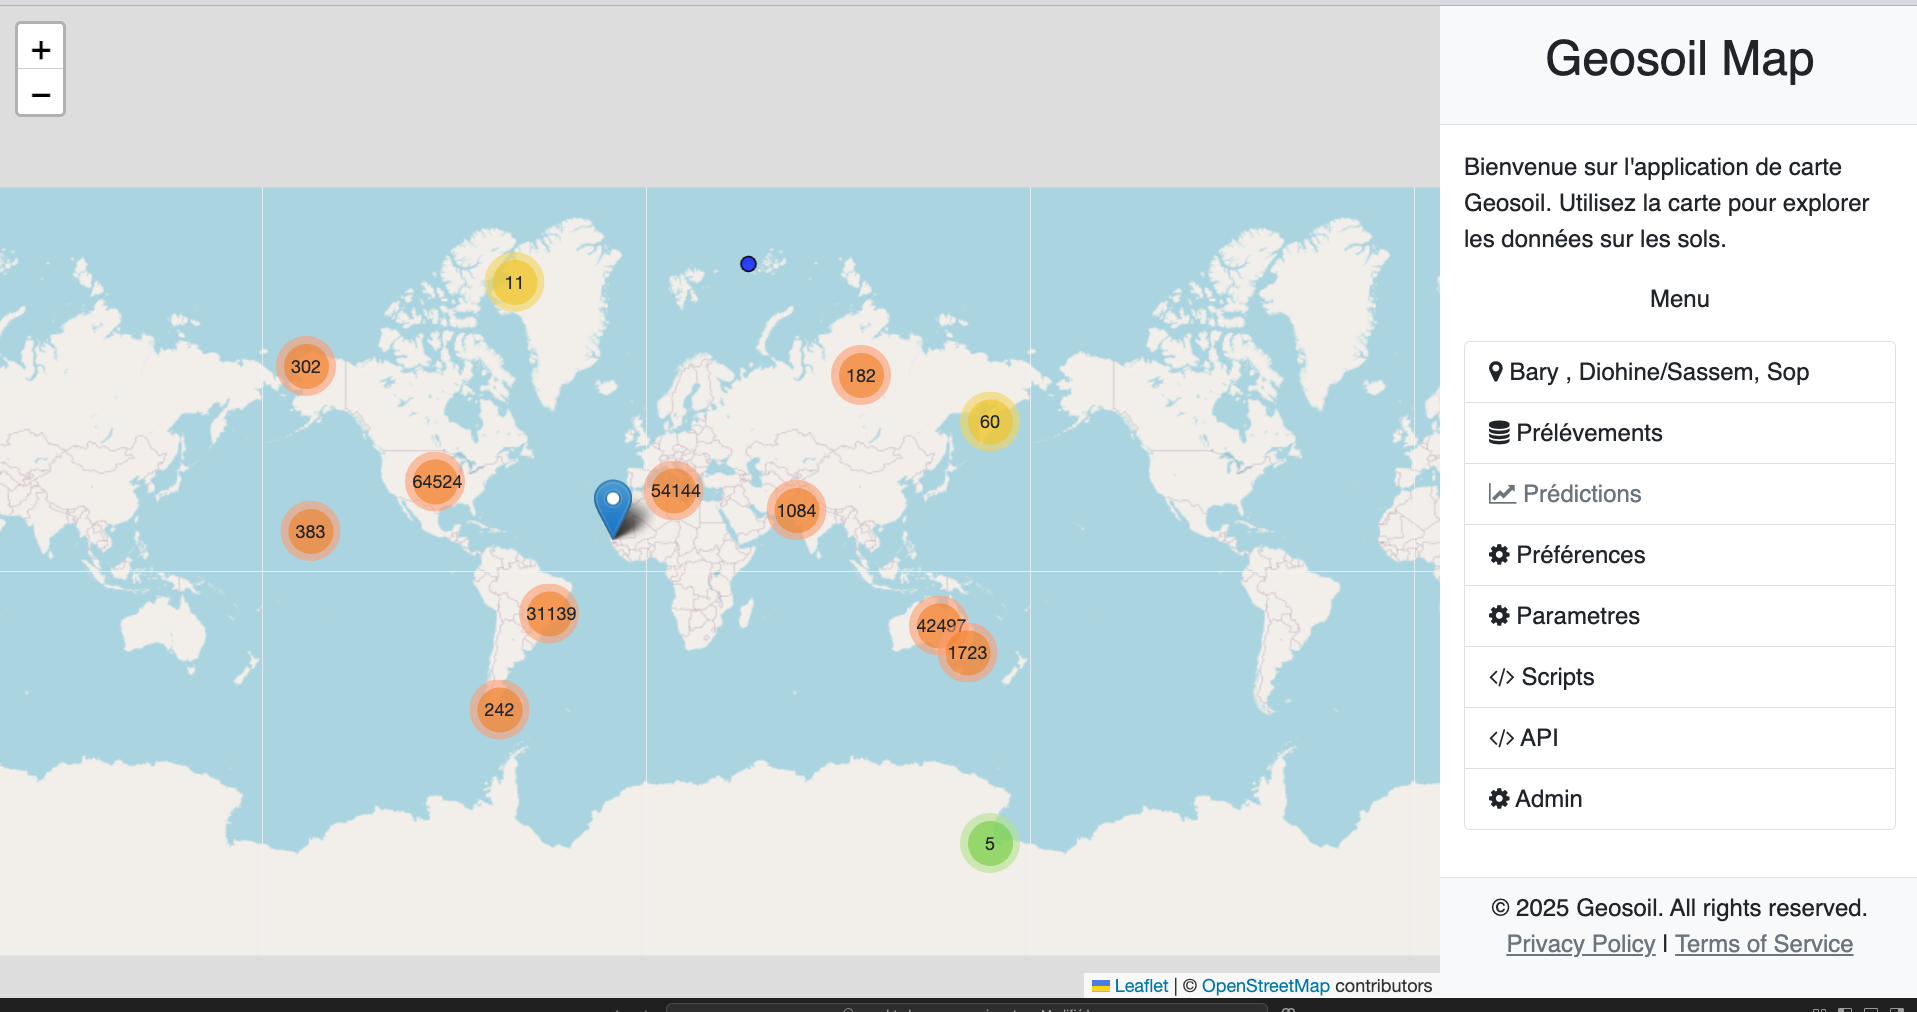
\includegraphics[width=.8\linewidth]{images/app.png}
      \caption{Page d'accueil.}
      \label{fig:app}
  \end{subfigure}
  \hfill
  \begin{subfigure}{0.48\textwidth}
      \centering
      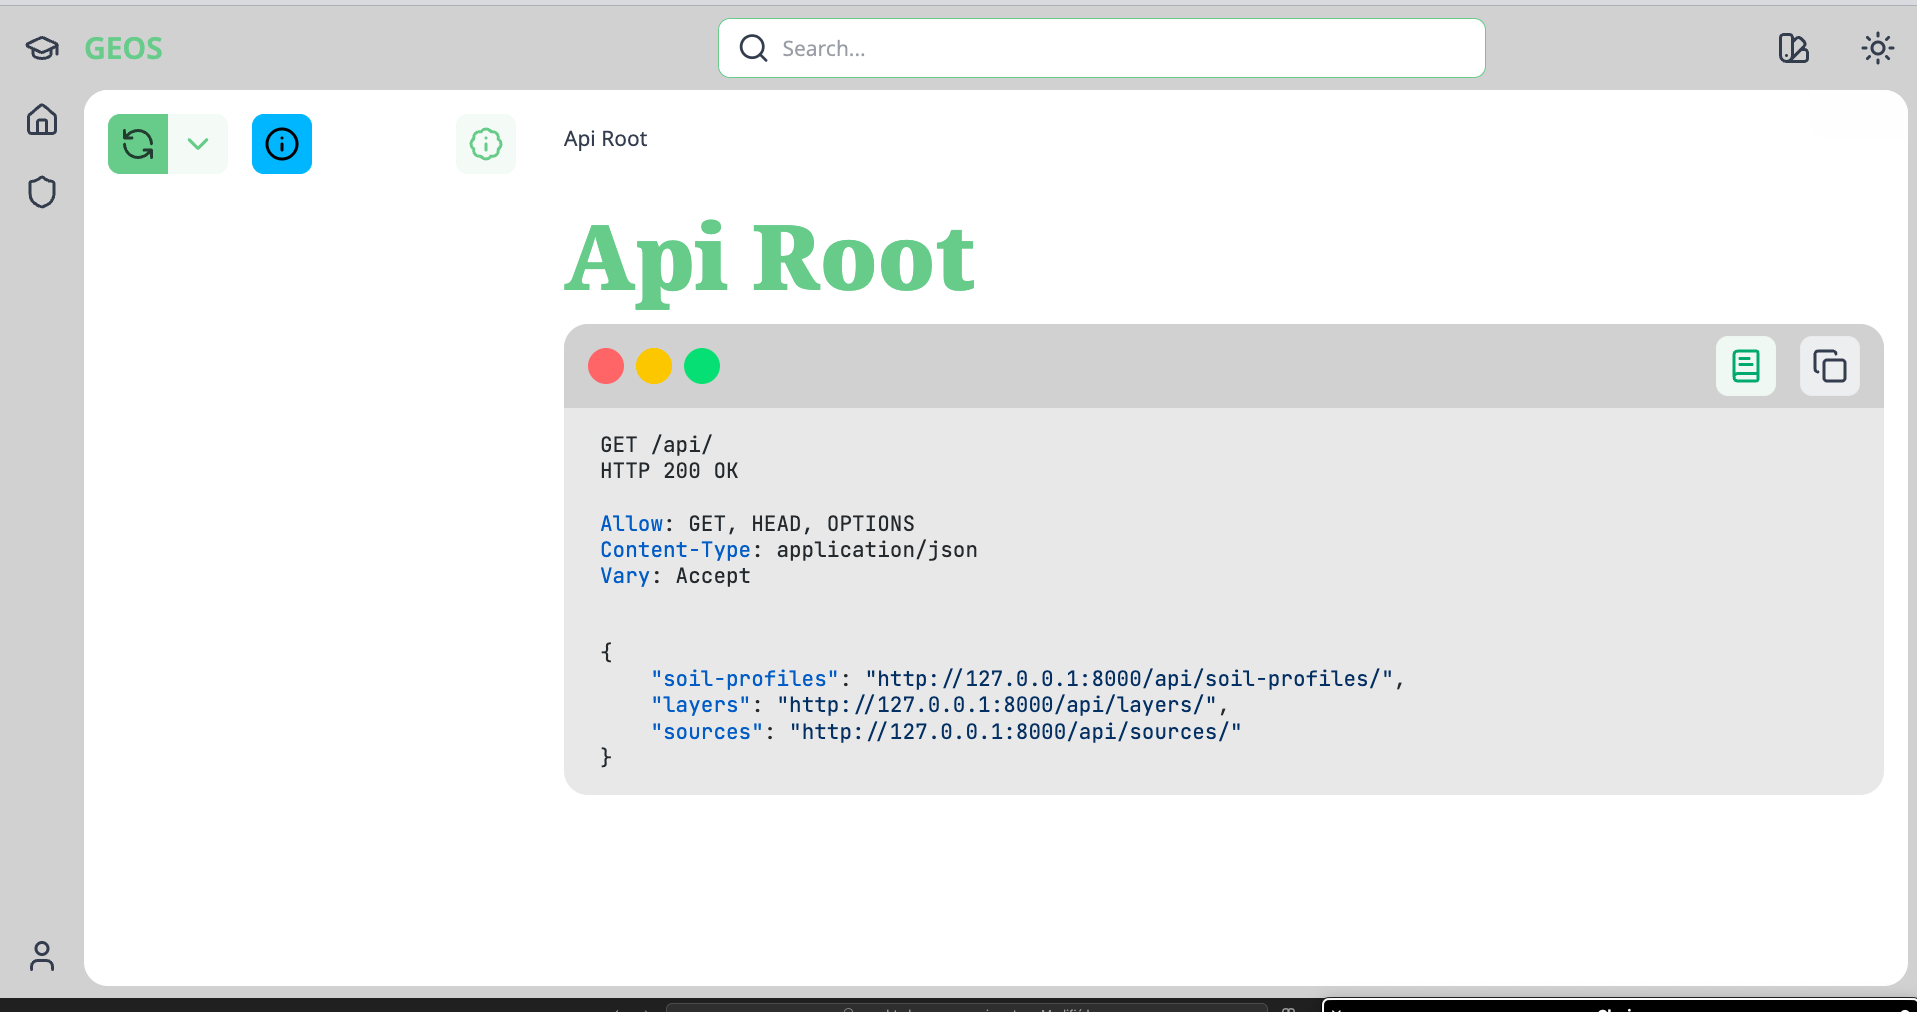
\includegraphics[width=.8\linewidth]{images/api.png}
      \caption{API.}
      \label{fig:api}
  \end{subfigure}
  \caption{Interface de l'application et API associée.}
  \label{fig:app_api}

\end{figure}


\section{Objectifs fonctionnels}
Le déploiement applicatif vise à rendre les résultats du modèle accessibles et exploitables par différents utilisateurs (chercheurs, décideurs, acteurs du développement rural). Les objectifs principaux sont :
\begin{itemize}
  \item Fournir une interface conviviale permettant de visualiser les cartes de stock de carbone organique du sol (SOC).
  \item Mettre à disposition une API permettant d’interroger le modèle sur de nouveaux points géolocalisés.
  \item Garantir la reproductibilité et la portabilité grâce à l’utilisation de conteneurs Docker.
  \item Assurer une intégration avec la base de données spatiale PostGIS pour stocker et gérer efficacement les données.
\end{itemize}

\section{Architecture (Django, PostGIS, API \texttt{/predict})}
L’architecture logicielle repose sur une application web développée avec le framework \textbf{Django} :
\begin{itemize}
  \item \textbf{Backend Django} : gestion des requêtes, communication avec la base de données et orchestration des prédictions.
  \item \textbf{Base de données PostGIS} : stockage des profils de sol, des covariables spatiales et des résultats de prédiction.
  \item \textbf{API REST /predict} : service qui prend en entrée des coordonnées géographiques et renvoie la prédiction du SOC avec un intervalle de confiance.
  \item \textbf{Frontend} : interface cartographique interactive (Leaflet/Mapbox) permettant de naviguer, zoomer et interroger les cartes.
  \item \textbf{Conteneurisation Docker} : chaque composant (Django, PostgreSQL/PostGIS, worker ML) est isolé et orchestré pour simplifier le déploiement.
\end{itemize}

% Schéma possible : Backend (Django) ↔ PostGIS ↔ API /predict ↔ Frontend cartographique

\section{Sécurité, performances et limites}
\subsection*{Sécurité}
\begin{itemize}
  \item Authentification par jetons (JWT) pour l’accès à l’API.
  \item Configuration SSL/TLS pour sécuriser les échanges.
  \item Gestion des droits utilisateurs (lecture seule pour les décideurs, écriture pour les chercheurs).
\end{itemize}

\subsection*{Performances}
\begin{itemize}
  \item Mise en cache des prédictions fréquentes pour réduire la latence.
  \item Optimisation des requêtes spatiales PostGIS (indexation GiST et BRIN).
  \item Possibilité de paralléliser l’inférence via des workers ML.
\end{itemize}

\subsection*{Limites}
\begin{itemize}
  \item Dépendance à la connectivité Internet pour l’accès à l’application.
  \item Coût computationnel élevé pour l’inférence sur de grandes surfaces en haute résolution.
  \item Nécessité de mettre à jour régulièrement les modèles avec de nouvelles données de sols et images satellitaires.
\end{itemize}


% ===================== Chapitre 8 =====================

\chapter{Conclusion et perspectives}

\section{Bilan des contributions}
Ce stage a permis de concevoir et d’expérimenter un pipeline complet, reproductible et opérationnel pour la prédiction du stock de carbone organique du sol (SOC) dans trois villages pilotes du Sénégal (Bary, Diohine/Sassem et Sop).

Les principales contributions sont :
\begin{itemize}
  \item Intégration multi-sources : combinaison de données pédologiques locales (IRD), continentales (AfSP) et globales (WoSIS), enrichies par l’imagerie Sentinel-2 et Landsat-8 ainsi que des covariables topographiques et pédologiques globales.

  \item Évaluation comparative : mise en œuvre et comparaison de plusieurs modèles de prédiction (Random Forest, XGBoost, Gradient Boosting, HistGradientBoosting, MLP PyTorch), avec des protocoles stricts de validation spatiale (GroupKFold et Leave-Area-Out).

  \item Innovation méthodologique : introduction d’une prédiction hiérarchique (SOC10 → SOC30) et de modèles par site, afin d’améliorer la robustesse sur les couches profondes et capturer les spécificités locales.

  \item Cartographie d’incertitude : production de cartes probabilistes (écart-type, intervalles de confiance à 90 %) pour accompagner les cartes prédictives et appuyer les décisions.

  \item Déploiement applicatif : développement d’une application web (Django + PostGIS) intégrant une API /predict et une interface cartographique interactive, permettant un accès pratique et reproductible aux résultats.

\end{itemize}

Ces contributions confirment la pertinence des approches d’apprentissage automatique, en particulier des réseaux de neurones entraînés localement, pour la cartographie fine et fiable du SOC en contexte sahélien.



\section{Limitations identifiées  }
Plusieurs contraintes méthodologiques et structurelles ont été mises en évidence :
\begin{itemize}
  \item Décalage temporel entre les profils pédologiques historiques (AfSP, WoSIS) et les séries satellites récentes (Sentinel-2, Landsat-8), réduisant la pertinence du transfert continental → local.

  \item Difficulté accrue pour la couche 10--30 cm, où la sensibilité des capteurs optiques diminue, entraînant une baisse de performance (\( R^2 \approx 0.65 \) contre \( 0.80 \) en surface).

  \item Distribution hétérogène des données : la densité limitée des profils IRD (\( 1\,800 \) profils concentrés sur trois villages) crée des biais spatiaux et accroît l’incertitude dans certaines zones.
\end{itemize}

Contraintes computationnelles : les modèles avancés (MLP) nécessitent des ressources GPU importantes, ce qui limite leur application à de très grandes surfaces.

\section{Perspectives scientifiques et opérationnelles}
À la lumière de ces résultats et limites, plusieurs axes d’amélioration se dégagent :

\begin{itemize}
  \item Alignement temporel des données : planifier de nouvelles campagnes de prélèvements pédologiques synchronisées avec les séries satellitaires récentes, afin de renforcer la cohérence spatio-temporelle.

  \item Enrichissement des covariables : intégrer des données hyperspectrales (PRISMA, EnMAP) et radar (Sentinel-1) pour améliorer la prédiction, notamment en profondeur.

  \item Approches hybrides : combiner apprentissage automatique et géostatistique (krigeage résiduel, co-krigeage) pour mieux capturer la structure spatiale.

  \item Méthodes avancées d’incertitude : recourir à des approches bayésiennes plus robustes ou à des modèles probabilistes (Gaussian Processes) pour fournir des cartes de confiance plus fines.

  \item Extension territoriale : appliquer le pipeline à d’autres territoires agricoles du Sénégal, voire de l’Afrique de l’Ouest, afin de produire des cartes régionales utiles aux décideurs publics et aux agriculteurs.

  \item Renforcement de l’interopérabilité : maintenir et enrichir l’application web pour en faire un outil partagé entre chercheurs, institutions agricoles et acteurs du développement rural.
\end{itemize}
\section{Conclusion générale}

En définitive, ce travail démontre qu’il est possible de construire un pipeline robuste, reproductible et opérationnel pour la prédiction du carbone organique du sol en contexte sahélien.
Il apporte à la fois :
\begin{itemize}
  \item une contribution scientifique, en confirmant la supériorité des approches d’apprentissage automatique (MLP, validations spatiales strictes),

  \item une contribution méthodologique, avec l’introduction de nouvelles approches (prédiction hiérarchique, validation LAO, cartographie d’incertitude),

  \item et une contribution opérationnelle, grâce au développement d’une application web interactive.

\end{itemize} 
Ce mémoire constitue ainsi une base solide pour le développement d’outils d’aide à la décision en matière de gestion durable des sols et de planification agricole, contribuant à la sécurité alimentaire et à l’adaptation au changement climatique en Afrique de l’Ouest.

\appendix
\chapter*{Annexes}
\addcontentsline{toc}{chapter}{Annexes}

% lien vers github
\section*{Code source}
\addcontentsline{toc}{section}{Code source}
Le code source complet du pipeline, incluant l’extraction des données, la préparation, l’entraînement des modèles, la quantification de l’incertitude et le déploiement applicatif, est disponible sur GitHub : \url{https://github.com/venire-ute/stage-rendu}
\nocite{*}
\printbibliography

\end{document}
